% ------------------------------------------------------------------------------
% Risk Modeller's Toolkit (RMTK) User Guide
%
% Authors:
% 	C. Casotto	- GEM Model Facility, Pavia, Italy
%
% Document distributed under the Common Creative License
% © GEM Foundation, Pavia, February 2014

%-------------------------------------------------------------------------------
%	LOAD PACKAGES
%-------------------------------------------------------------------------------
%%%%%%%%%%%%%%%%%%%%%%%%%%%%%%%%%%%%%%%%%
% The Legrand Orange Book
% LaTeX Template
% Version 1.4 (12/4/14)
%
% This template has been downloaded from:
% http://www.LaTeXTemplates.com
%
% Original author:
% Mathias Legrand (legrand.mathias@gmail.com)
%
% License:
% CC BY-NC-SA 3.0 (http://creativecommons.org/licenses/by-nc-sa/3.0/)
%
% Compiling this template:
% This template uses biber for its bibliography and makeindex for its index.
% When you first open the template, compile it from the command line with the 
% commands below to make sure your LaTeX distribution is configured correctly:
%
% 1) pdflatex rmtk-docs
% 1a) pdflatex -shell-escape rmtk-docs
% 2) makeindex rmtk-docs.idx -s StyleInd.ist
% 3) biber rmtk-docs
% 4  makeglossaries rmtk-docs
% 4) pdflatex rmtk-docs x 2
%
% After this, when you wish to update the bibliography/index use the appropriate
% command above and make sure to compile with pdflatex several times 
% afterwards to propagate your changes to the document.
%
% This template also uses a number of packages which may need to be
% updated to the newest versions for the template to compile. It is strongly
% recommended you update your LaTeX distribution if you have any
% compilation errors.
%
% Important note:
% Chapter heading images should have a 2:1 width:height ratio,
% e.g. 920px width and 460px height.
%
%%%%%%%%%%%%%%%%%%%%%%%%%%%%%%%%%%%%%%%%%

%----------------------------------------------------------------------------------------
%	PACKAGES AND OTHER DOCUMENT CONFIGURATIONS
%----------------------------------------------------------------------------------------

\documentclass[11pt,fleqn]{book} % Default font size and left-justified equations

\usepackage[top=3cm,bottom=3cm,left=3.2cm,right=3.2cm,headsep=10pt,a4paper]{geometry} % Page margins

\usepackage{xcolor} % Required for specifying colors by name
\definecolor{ocre}{RGB}{243,102,25} % Define the orange color used for highlighting throughout the book

% Font Settings
\usepackage{avant} % Use the Avantgarde font for headings
%\usepackage{times} % Use the Times font for headings
\usepackage{mathptmx} % Use the Adobe Times Roman as the default text font together with math symbols from the Sym­bol, Chancery and Com­puter Modern fonts

\usepackage{microtype} % Slightly tweak font spacing for aesthetics
\usepackage[utf8]{inputenc} % Required for including letters with accents
\usepackage[T1]{fontenc} % Use 8-bit encoding that has 256 glyphs

% Bibliography
\usepackage{csquotes}
\usepackage[style=alphabetic,
            sorting=nyt,
            sortcites=true,
            natbib=true,
            style=authoryear,
            maxcitenames=2,
            maxbibnames=100,
            autopunct=true,
            babel=hyphen,
            hyperref=true,
            doi=true,
            abbreviate=false,
            backref=true,
            backend=biber,
	    	uniquename=false,
	    	uniquelist=false]{biblatex}
\addbibresource{./bibliography/rmtk.bib} % BibTeX bibliography file
\defbibheading{bibempty}{}

% Figure caption settings
\usepackage[textfont=it,margin=10pt,font=small,labelfont=bf,labelsep=endash]{caption}
\usepackage{subcaption}
\usepackage{rotating}

% Table - colors from
\usepackage{verbatim}
\usepackage{color, colortbl}
\definecolor{almond}{rgb}{0.94, 0.87, 0.8}
\definecolor{ashgrey}{rgb}{0.7, 0.75, 0.71}
\definecolor{anti-flashwhite}{rgb}{0.95, 0.95, 0.96}
\definecolor{airforceblue}{rgb}{0.36, 0.54, 0.66}

% Index
\usepackage{calc} % For simpler calculation - used for spacing the index letter headings correctly
\usepackage{makeidx} % Required to make an index
% \setcounter{tocdepth}{3}    % entries down to \subsubsections in the TOC
\makeindex % Tells LaTeX to create the files required for indexing

\usepackage{todonotes}
\usepackage{geometry}
\usepackage{marginnote}

%
% Package to create a glossary - It must be uploaded after hyperref
% to produce the glossary: makeglossaries OQB
\usepackage[acronym,nonumberlist,style=altlist]{glossaries}
\glstoctrue
\makeglossaries

% package for bold symbols
\usepackage{bm}

% for better looking tables
\usepackage{ctable}
\usepackage{microtype}

% for listing Python code
\usepackage{listings}

%
%----------------------------------------------------------------------------------------
% Trees
%\usepackage[pdf]{pstricks}
%\usepackage{auto-pst-pdf}
%\usepackage{pst-tree}
%


%-------------------------------------------------------------------------------
% Insert the structure.tex file which contains the majority of the structure 
% behind the template
\input{./configuration/structure.tex}


% =============================================================== BEGIN DOCUMENT
\begin{document}
\lstset{language=Python} % --------------- For listings environment - use python
% OpenQuake Book Glossary 
% To cite a glossary element in a document:
%	\gls{seismicsourcedata}
%	\Gls{seismicsourcedata} - First initial is uppercase
%	\GLS{seismicsourcedata} - All initials are uppercase
%	\glspl{seismicsourcedata} - Plural
% To process the glossary:
% 	makeglossaries oqb

%
% ------- A
%
% ------- B
\newglossaryentry{branch}{
	name = branch,
	plural= branches,
	description={
	The simplest element in a logic tree; it belongs to a 
	\gls{branchset} where it represents one possible option among a finite 
	number of alternatives. A branch is associated with a weight 
	value \citep{scherbaum2011} if the \gls{branchset} represents the 
	epistemic uncertainty on a parameter or a model when the \gls{branchset} 
	is used to specify alternative models (e.g. district \glspl{acr:mfd})
	}
}
%
% ------- C
\newacronym{cpsha}{cPSHA}{Classical PSHA}
\newglossaryentry{configurationfile}{
	name =  configuration file,
	description = {
	Usually the file containing the information necessary to run a calculation
	in OpenQuake
	}
}
%
% ------- D
%
% ------- E
\newacronym{acr:erf}{ERF}{Earthquake\- Rup\-ture\- Forecast}
\newacronym{acr:epsha}{ePSHA}{Event-based PSHA}
%
\newglossaryentry{earthquakeruptureforecast}{
	name = earthquake rupture forecast,
	description={
	A list of all possible ruptures generated by all the sources included 
	in a seismic source model. Each element in the list contains: the rupture 
	geometry and the rupture probability of occurrence in a given time span. 
	%
	See also the definition available on the 
	\href{http://www.opensha.org/glossary-earthquakeRuptureForecast}
	{OpenSHA website}}
}
\newglossaryentry{earthquakeruptureforecastcalculator}{
	name = earthquake rupture forecast calculator,
	description={
	Calculator producing a \gls{seismicsourcemodel} from a 
	\gls{seismicsourcelogictree} 
	}
}
%
%
% ------- F
%
% ------- G
\newacronym{acr:gem}{GEM}{Global Earthquake Model}
\newacronym{acr:gmpe}{GMPE}{Ground Motion Prediction Equation}
\newacronym{acr:gsim}{GSIM}{Ground Shaking Intensity Model}
\newacronym{acr:gmm}{GMM}{Ground Motion Model}

\newglossaryentry{groundmotionfield}{
	name = ground-motion field,
	description={An object describing the geographic distribution around 
	a rupture of a ground motion intensity measure}
}
\newglossaryentry{groundmotionmodel}{
	name = ground-motion model,
	description={An object that given a rupture with specific properties
	computes the expected ground motion at the given site. In simplest case 
	a ground motion model corresponds to a \gls{groundmotionpredictioneq}. 
	In case of complex PSHA input models, the produced ground motion models 
	contains a set of \glspl{acr:gmpe}, one for each tectonic region considered.
	}
}
\newglossaryentry{groundmotionpredictioneq}{
	name = ground-motion prediction equation,
	description={
		An equation that - given some fundamental parameters characterizing 
		the source, the propagation path and the site (in the simplest 
		case magnitude, distance and V$_\text{S,30}$) - computes the 
		value $GM$ of a (scalar) ground motion intensity parameter.
	}
}
%
% ------- I 
\newacronym{acr:imt}{IMT}{Intensity Measure Type}
\newglossaryentry{investigationtime}{
	name = investigation time,
	description={The time interval considered to calculate hazard; usually 
	it corresponds to 50 years}
}
%
% ------- L
\newglossaryentry{logictree}{
	name = logic tree,
	description={Data structure used to systematically describe uncertainties
	on parameters and models used in a PSHA study}
}
%
% ------- M
%
% ------- O
\newacronym{acr:oq}{OQ}{OpenQuake}
\newacronym{acr:oqe}{OQ-engine}{OpenQuake-engine}
\newacronym{acr:oqhl}{OQ-hazardlib}{OpenQuake hazard library}
\newacronym{acr:oqrl}{OQ-risklib}{OpenQuake risk library}
%
% ------- N
\newacronym{acr:nrml}{NRML}{Natural hazard Risk Markup Language}
%
% ------- P
\newacronym{acr:pga}{PGA}{Peak Ground Acceleration}
\newacronym{acr:pgv}{PGV}{Peak Ground Velocity}
\newacronym{acr:psha}{PSHA}{Probabilistic Seismic Hazard Analysis}
\newacronym{acr:peer}{PEER}{Pacific Earthquake Engineering Center}
%
\newglossaryentry{psha}{
	name = probabilistic seismic hazard analysis, 
	description={A methodology to compute seismic hazard which takes into 
	account the contributions coming from all the sources of engineering 
    importance for a specified site}	
}
%
% ------- R
%
% ------- S
\newglossaryentry{softwarequalityassurance}{
	name = software quality assurance,
	description={
    Software quality assurance (SQA) consists of a means of monitoring 
    the software engineering processes and methods used to ensure quality.
    The methods by which this is accomplished are many and varied, and 
    may include ensuring conformance to one or more standards, such as 
    ISO 9000 or a model such as CMMI.
    SQA encompasses the entire software development process, which 
    includes processes such as requirements definition, software design, 
    coding, source code control, code reviews, software configuration 
    management, testing, release management, and product integration. 
    SQA is organized into goals, commitments, abilities, activities,
    measurements, and verifications.
	}
}
\newacronym{acr:sa}{S$_a$}{Spectral Acceleration}
%
% ------- T
%
% ------- U
\newacronym{acr:usgs}{USGS}{United States Geological Survey}
%
% ------- V  % ------------------------------  Load the glossary


%-------------------------------------------------------------------------------
%	TITLE PAGE
%-------------------------------------------------------------------------------

\begingroup
\thispagestyle{empty}
%\AddToShipoutPicture*{\put(6,5){\includegraphics[scale=1]{background}}} % Image background
\par\normalfont\fontsize{15}{15}\sffamily\selectfont
“OpenQuake: Calculate, share, explore”
\centering
\vspace*{9cm}
\par\normalfont\fontsize{35}{35}\sffamily\selectfont
Risk Modeller's Toolkit - User Guide\par % Book title
\endgroup

%----------------------------------------------------------------------------------------
%	COPYRIGHT PAGE
%----------------------------------------------------------------------------------------

\newpage
~\vfill
\thispagestyle{empty}

\noindent Copyright \copyright\ 2014 GEM Foundation\\ % Copyright notice

\noindent \textsc{Published by GEM Foundation}\\ % Publisher

\noindent \textsc{globalquakemodel.org/openquake}\\ % URL

\noindent
   {\textbf{Citation}} \hfill \\
   Please cite this document as:\\
   Casotto, C. (2014) OpenQuake Risk Modeller's Toolkit - User Guide. \textit{Global Earthquake Model (GEM). Technical Report}\\

   {\bf{Disclaimer}} \hfill \\
\noindent
   The ``Risk Modeller's Tookit - User Guide'' is distributed in the hope 
   that it will be useful, but without any warranty: without 
   even the implied warranty of merchantability or fitness for a 
   particular purpose. While every 
   precaution has been taken in the preparation of this document, in 
   no event shall the authors of the manual and the GEM Foundation be 
   liable to any party for direct, indirect, special, incidental, or 
   consequential damages, including lost profits, arising out of the 
   use of information contained in this document or from the use of 
   programs and source code that may accompany it, even if the authors 
   and GEM Foundation have been advised of the possibility of such damage. 
   The Book provided hereunder is on as "as is" basis, and the authors 
   and GEM Foundation have no obligations to provide maintenance, support,
   updates, enhancements, or modifications. 
   \hfill \\
   The current version of the book has been revised only by members of 
   the GEM model facility and it must be considered a draft copy. 
   %
   \vspace{0.4cm} \hfill \\
   {\bf{License}} \hfill \\
   This Book is distributed under the Creative Common License 
   Attribution-NonCommercial-NoDerivs 3.0 Unported (CC BY-NC-ND 3.0) 
   (see link below). You can download this Book and share it with 
   others as long as you provide proper credit, but you cannot change 
   it in any way or use it commercially. 
   \hfill \\

\noindent \textit{First printing, November 2014} % Printing/edition date

%----------------------------------------------------------------------------------------
%	TABLE OF CONTENTS
%----------------------------------------------------------------------------------------

\chapterimage{./figures/chapter_head_1.pdf} % Table of contents heading image

\pagestyle{empty} % No headers

\tableofcontents % Print the table of contents itself

\cleardoublepage % Forces the first chapter to start on an odd page so it's on the right

\pagestyle{fancy} % Print headers again

%----------------------------------------------------------------------------------------
%	PREAMBLE
%----------------------------------------------------------------------------------------
\chapterimage{./figures/chapter_head_2.pdf} % Chapter heading image
\chapter*{Preface}
\addcontentsline{toc}{chapter}{Preamble}
The goal of this book is to provide a comprehensive and transparent description
of the methodologies adopted and implemented in the Risk Modeller's Toolkit
(RMTK).
% Add short description about RMTK

% Add short description about main contributors
It is freely distributed under an Affero GPL license 
(more information available at this link 
\href{http://www.gnu.org/licenses/agpl-3.0.html}{http://www.gnu.org/licenses/agpl-3.0.html})

%----------------------------------------------------------------------------------------
%	CHAPTER 1
%----------------------------------------------------------------------------------------
\chapterimage{./figures/chapter_head_2.pdf} % Chapter heading image
\chapter{Introduction}
\label{chap:introduction}
\section{Introduction}
The Risk Modeller's Toolkit (\textit{rmtk} hereafter) is a Python 2.7 library of functions written by scientists at the GEM Model Facility, which is intended to provide scientists and engineers with the tools to help creating the vulnerability input models that go into the OpenQuake risk engine and managing the generated output files. The intention of this software is to provide scientists and engineers with the means to apply some of the most commonly used algorithms for preparing vulnerability models using structural analysis data and to facilitate the visualisation and the use of the outputs from OpenQuake. In forthcoming versions will hope to make available more methodologies for the process indicated here, and to integrate new functionalities for i) building structural models of different levels of complexity within the \textit{rmtk} in combination with a structural analysis software, ii) running dynamic and static analysis within the \textit{rmtk} in combination with a structural analysis software, iii) deriving vulnerability curves directly applying engineering demand parameters-to-loss functions to structural analysis results.

\subsection{Getting Started and Running the Software}
The Modeller’s Toolkit is designed for execution from the command line. As with OpenQuake engine, the preferred environment is Ubuntu Linux (12.04 or later), however, the \textit{rmtk} is a library that can be run using any python environment for other operating systems (i.e. Mac, Windows). A careful effort has been made to keep the number of additional dependencies to a minimum. No packaged version of the software has been released at the time of writing, so the user must install Python 2.7 and the dependencies manually. The current dependencies are:
\begin{itemize}
\item Numpy and Scipy (included in the standard OpenQuake installation)
\item Matplotlib (http://matplotlib.org/)
\item Os
\end{itemize}

The Numpy, Scipy, Matplotlib, and Os dependencies are installed in the library for the demos, but once Python 2.7 has been installed they can be easily installed from the command line by:

\begin{Verbatim}[frame=single, commandchars=\\\{\}, samepage=true]
~\$ sudo pip install numpy
~\$ sudo pip install scipy
~\$ sudo pip install matplotlib
~\$ sudo pip install os
\end{Verbatim}

To enable usage of the \textit{rmtk} within any location in the operating system, OSX and Linux users should add the folder location (set the path) manually to the command line profile file. This can be done as follows:
\begin{enumerate}
\item Using a command line text editor (e.g. VIM), open the ~/.profile folder as follows:

\begin{Verbatim}[frame=single, commandchars=\\\{\}, samepage=true]
~\$ vim ~/.profile
\end{Verbatim}

\item At the bottom of the profile file (if one does not exist it will be created) add the line:

\begin{Verbatim}[frame=single, commandchars=\\\{\}, samepage=true]
export PYTHONPATH=/path/to/rmtk/folder/:\$PYTHONPATH
\end{Verbatim}

Where \verb=/path/to/rmtk/folder/= is the system path to the location of the \textit{rmtk} folder (use the command \verb=pwd= from within the \textit{rmtk} folder to view the full system path).

\item Re-source the bash shell via the command

\begin{Verbatim}[frame=single, commandchars=\\\{\}, samepage=true]
~\$ source ~/.profile
\end{Verbatim}
 
\end{enumerate}

\subsubsection{Windows Installation}

Although this installation has been primarily tested in a Linux/Unix environment it is possible to install natively in Windows using the following process. This assumes that no other version of Python is installed in your windows environment.

The easiest way to install all of the dependencies needed is by virtue of the PythonXY program \href{http://code.google.com/p/pythonxy/}{http://code.google.com/p/pythonxy/}, a free and open python user interface, which will bring in all the dependencies nedeed automatically. The installer for the latest version of PythonXY can be downloaded from here: \href{http://code.google.com/p/pythonxy/wiki/Downloads?tm=2}{http://code.google.com/p/pythonxy/wiki/Downloads?tm=2}.

Click on the executable and follow the instructions (the installation may take up to half an hour or more, depending on the system). It is strongly recommended that the use opt for the ``\textbf{FULL}'' installation, which should bring in all of the dependencies needed for the \textit{rmtk}. 

Now, download the zipped folder of the \textit{rmtk} from the github repository and unzip to a folder of your choosing. To allow for usage of the \textit{rmtk} throughout your operating system, do the following: 

\begin{enumerate}
\item From the desktop, right-click \textbf{My Computer} and open \textbf{Properties}
\item In the ``System Properties'' window click on the \textbf{Advanced} tab.
\item From the ``Advanced'' section open the \textbf{Environment Variables}.
\item In the ``Environment Variables'' you will see a list of ``System Variables'', select ``Path'' and ``Edit''.
\item Add the path to the \textit{rmtk} directory to the list of folders then save.
\end{enumerate}

After this process it may be necessary to restart PythonXY.



	% \section{Motivation}
	% \label{sec:motivation}
	% 	\input{tex/motivation}

	\section{Organization}
	\label{sec:organization}
	This manual is designed to explain the various functions in the toolkit, to provide the theoretical background behind them, and to guide the modeller in the use of the rmtk within the ``IPython Notebook'' environment. This novel tool implements Python inside a web-browser environment, permitting the user to execute real Python workflows, whilst allowing for images and text to be embedded. Its use is encouraged especially for beginner python users for a more visual application of the rmtk.

The IPython Notebook  comes installed from version 1.0 of IPython, that can be installed from the python package repository by entering: 

\begin{Verbatim}[frame=single, commandchars=\\\{\}, samepage=true]
~\$ sudo pip install ipython
\end{Verbatim}

A notebook session can be started via the command:

\begin{Verbatim}[frame=single, commandchars=\\\{\}, samepage=true]
~\$ ipython notebook --pylab inline
\end{Verbatim}

The tutorial itself does not specifically require a working knowledge of Python. However, an understanding of the basic python data types is highly desirable. Users who are new to Python are recommended to familiarise themselves with Appendix \ref{sec:python_guide} of this tutorial. 

The \textit{rmtk} is currently subdivided into two classes of tools, the Vulnerability and Plotting tools, presented in Chapter 2 and Chapter 3 of this tutorial respectively. In the Vulnerability chapter the vulnerability methodologies implemented are classified in Non-linear Static (NLS) and Non-linear Dynamic (NLD) according to the structural analysis type performed to assess the response of the building. These two main sections (NLS and NLD) are organised as follows:

\begin{itemize}
\item General Introduction.
\item Getting Started, where it is explained what files need to be executed to start the vulnerability analysis, and what options are available to call the preferred methodology and to input the preferred data type.
\item Description of the methodologies.
\end{itemize}

Within the description of each methodology the user can find the following subsections:
\begin{itemize}
\item Theoretical description of the method.
\item Description and examples of the inputs.
\item Description of the workflow.
\end{itemize}

A summary of the algorithms available in the present version is given in Table \ref{tab:current_features}.
\begin{table}[!htbp]
\centering
\begin{tabular}{|c|c|} \hline
Feature & Algorithm\\ \hline
\textbf{Non-linear Static} & Cr-based (\cite{Ruiz-Garcia and Miranda, 2007})\\
    & Spo2ida (\cite{Vamvatsikos and Cornell, 2006}) \\
    & R-$/mu$-T-based (\cite{Dolsek and Fajfar, 2004}) \\ \hline
 \textbf{Non-linear Dynamic} & DPM-based (\cite{Silva et al., 2013})\\
  & Ida-postprocessing (\cite{Vamvatsikos and Cornell, 2002}) \\ \hline
\end{tabular}
\caption{Current algorithms in the HMTK}
\label{tab:current_features}
\end{table}



%----------------------------------------------------------------------------------------
%	CHAPTER 2
%----------------------------------------------------------------------------------------
\chapterimage{./figures/chapter_head_2.pdf} % Chapter heading image
\chapter{Vulnerability}
\label{chap:vulnerability}
\input{./tex/vulnerability}

	\section{Non-linear Static (NLS) Methods}
	\label{sec:nls-intro}
	Nonlinear Static Methods are based on the use of capacity curves, resulting from nonlinear static pushover analysis, to determine the median seismic intensity values $\hat{s}_c$ corresponding to the attainment of a certain damage state threshold (limit state) and the corresponding dispersion $\beta_{sc}$. These parameters are used to represent a fragility curve as the probability of the limit state capacity C being exceeded by the demand D, both expressed in terms of intensity levels (s$_c$ and s respectively), as shown in the following equation:

\begin{equation}
P_{LS}(s) = P(C < D | s) = \Phi(\frac{ln s -ln \hat{s}_c}{\beta_{sc}})
\label{eq:fragility-definition}
\end{equation}

The methodologies implemented so far in the RMTK allow to consider different shapes of the pushover curve, multilinear and bilinear, record-to-record dispersion and dispersion in the damage state thresholds in a systematic and harmonised way. 

Different input types can be inserted depending on whether the user has already at his disposal an idealised pushover curve or it has to be derived from the raw results of a pushover analysis. Fragility and vulnerability functions can be derived for a single building or for a class of buildings.

The intensity measure to be used is S$_a$ and a mapping between any engineering demand parameter (EDP), assumed to describe the damage state thresholds, and the roof displacement should be available from the pushover analysis.

Ruiz-Garcia and Miranda (2007) study on inelastic displacement demand estimation, Vamvatsikos and Cornell (2006) and Dolsek and Fajfar (2004) work on seismic demand estimation with multilinear static pushover curves, have been integrated in three nonlinear static procedures, C$_R$-based, spo2ida-based and R-$mu$-T-based. In this way the user has the chance to select the procedure consistent with the available input, the type of structural analyses performed, the type of structures and the type of vulnerability assessment to perform. 

In section \ref{subsec:nls-how-to-use} the main information necessary to start the analysis are presented. In sections \ref{subsec:nls-ruiz-garcia-miranda}, \ref{subsec:nls-spo2ida} and \ref{subsec:nls-dolsek-fajfar} the three procedures are explained respectively, from the point of view of the scientific background behind the metho and their step-by-step implementation in the python script.

		\subsection{Using the NLS module}
		\label{subsec:nls-how-to-use}
		To start using the nonlinear static procedure with record-to-record variability a command line text editor should be used to enter manually the folder location where the \textit{rmtk} has been saved, as shown in the example below:

\begin{Verbatim}[frame=single, commandchars=\\\{\}, samepage=true]
~\$ cd path/to/rmtk/folder/rmtk/vulnerability
\end{Verbatim}

Where /path/to/rmtk/folder/ is the system path to the location of the \textit{rmtk} folder. From the text editor iPython browser page can be opened with the following command line:

\begin{Verbatim}[frame=single, commandchars=\\\{\}, samepage=true]
~\$ ipython-2.7 notebook --pylab=inline
\end{Verbatim}

Once the iPython page is opened on the browser, the python scripts contained in the \textit{vulnerability} directory will be visible. The file \textit{NSM\_dispersion.ipynb} should be selected to start the calculations.

In the initial section of the script "Define Options" the user should set the options, while the input corresponding to the defined options should be entered in the folder \textit{NSP/input}. The main options to define are the following:

\begin{itemize}
\item Type of procedure: either C$_R$-based, spo2ida-based or R-$\mu$-T-based. The main difference between the three is that C$_R$-based procedure is applicable to elasto-plastic idealised capacity curve only, while spo2ida-based and R-$\mu$-T-based procedure fit any kind of multilinear curve.
\item Type of input: either results of a pushover analysis in terms of displacement vs base shear at each time step or idealised pushover curve, as shown in Figures \ref{fig:expPushover} and \ref{fig:expIdealised}.

\begin{figure}[!htbp]
\centering
\includegraphics[width=10cm]{./figures/PushoverCurve.png}
\caption{Pushover curve.}
\label{fig:expPushover}
\end{figure}

\begin{figure}[!htbp]
\centering
\includegraphics[width=10cm]{./figures/IdealisedCurve.png}
\caption{Idealised pushover curve.}
\label{fig:expIdealised}
\end{figure}

\item Type of output: either fragility curve (probability of exceedance of a set of limit states vs seismic intensity, as shown in Figure \ref{fig:expFragility}) or vulnerability curve (loss ratio vs seismic intensity, as shown in Figure \ref{fig:expVulnerability}).
\end{itemize}

\begin{figure}[!htbp]
\centering
\includegraphics[width=10cm]{./figures/fragility.png}
\caption{Output: fragility curve}
\label{fig:expFragility}
\end{figure}

\begin{figure}[!htbp]
\centering
\includegraphics[width=10cm]{./figures/vulnerability.png}
\caption{Output: vulnerability curve}
\label{fig:expVulnerability}
\end{figure}

The outputs are available in the \textit{outputs} folder, located in the \textit{vulnerability} directory. The nonlinear static procedures with dispersion produces results in terms of spectral acceleration in units of g.\\
These options and others need to be defined in the initial section of the script "Define Options". In section \ref{subsubsec:options} the alternatives values that the initial variables can assume and their meaning are described in detail, while the parameters to be inserted in the input files are listed below. They are fully described in section \ref{subsec:nls-ruiz-garcia-miranda} section \ref{subsec:nls-spo2ida} and section  \ref{subsec:nls-dolsek-fajfar}, within the presentation of each procedure.

\subsubsection{Options}
\label{subsubsec:options}
The type of procedure to be performed and the type of inputs at disposal, are set with the variables \textit{an\_type} and \textit{in\_type} respectively. With the variable \textit{an\_type} the user can choose between:

\begin{Verbatim}[frame=single, commandchars=\\\{\}, samepage=true]
an\_type = 0 # Cr-based procedure (Ruiz-Garcia and Miranda, 2007)
an\_type = 1 # spo2ida-based procedure (Vamvatsikos and Cornell, 2006)
an\_type = 2 # R-m-T-based procedure (Dolsek and Fajfar, 2004)
\end{Verbatim}

With the variable \textit{in\_type} the user can choose between:

\begin{Verbatim}[frame=single, commandchars=\\\{\}, samepage=true]
in\_type = 0 # idealised pushover curve
in\_type = 1 # raw results from a pushover analysis
\end{Verbatim}

The variable \textit{vuln} instead gives the opportunity to decide the type of outputs, whether to stop the process at the derivation of the fragility curves, or to go all the way up to the vulnerability curve definition, applying damage-to-loss functions.

\begin{Verbatim}[frame=single, commandchars=\\\{\}, samepage=true]
vuln = 0 # derive fragility curves 
vuln = 1 # derive vulnerability curve
\end{Verbatim}

The variable \textit{g} serves the purpose of defining the units that are used. A floating number must be assigned to the gravity acceleration, compatible with the units used for the period of vibration and for the displacements (if the period is expressed in seconds and displacements are in meters, then g = 9.81). The variable \textit{iml} is a numpy array that identifies the intensity measure levels for which loss ratios are computed and provided in the vulnerability curve. The variable \textit{MC} defines the number of Monte Carlo simulations to account for uncertainty in the damage thresholds.

\begin{Verbatim}[frame=single, commandchars=\\\{\}, samepage=true]
g = 9.81
iml = np.linspace(0.1,15,100)
MC = 25
\end{Verbatim}

The variable \textit{plotflag} allows or inhibits the displaying of plots. It is a python list composed of 4 integers, each one controlling a different plot: idealised pushover curve, 16\%-50\%-84\% ida curves, fragility curves and vulnerability curve respectively. Each integer can take as value either zero or one, whether the corresponding graph has to be displayed or not:

\begin{Verbatim}[frame=single, commandchars=\\\{\}, samepage=true]
plotflag = [1, 1, 1, 1] # plot all the graphs
plotflag = [0, 0, 0, 0] # do not plot any graph
\end{Verbatim}

The following variables set some of the characteristics of the plots:

\begin{itemize}
\item \textit{linew}: integer for defining lines width.
\item \textit{fontsize}: fontsize used for labels, graphs etc.
\item \textit{units}: list of 3 strings defining displacements, forces and Spectral acceleration units, as ['[kN]', '[m]', '[m/s$^2$]'], to be displayed on the axes of the plots.
\end{itemize}

The last set of variables is needed for R-$\mu$-T-based procedure only:
\begin{itemize}
\item \textit{Tc}: constant accel-constant velocity corner period of a Newmark-Hall type spectrum. Default value is 0.5.
\textit{Td}: constant velocity-constant displacement corner period of a Newmark-Hall type spectrum. Default value is 1.8.
\end{itemize}


		\subsection{C$_R$-based procedure (Ruiz-Garcia and Miranda, 2007)}
		\label{subsec:nls-ruiz-garcia-miranda}
		The aim of this procedure, proposed by Vamvatsikos (2014), is the estimation of the median spectral acceleration value $\hat{S}_{a,ds}$, that brings the structure to the attainment of a set of damage states \textit{ds}, and the corresponding dispersion beta $\beta_{S_a}$, the parameters needed for the mathematical representation of fragility in equation \ref{eq:fragility-definition}. The aim is achieved making use of the work by Ruiz-Garcia and Miranda (2007), where the inelastic displacement demand of bilinear SDoF systems is related to the elastic displacement with a simple relationship.

The C$_R$-based procedure presented herein is applicable to bilinear elasto-plastic capacity curve only, and it is suitable for single building fragility curve estimation, as described in section \ref{subsubsec:single-building}. However the fragility curves derived for single buildings can be combined in a unique fragility curve, which considers also the inter-building uncertainty, as described in the following sections.

\subsubsection{Single Building Fragility and Vulnerability function}
\label{subsubsec:single-building}
This procedure provides a simple relationship between median damage state threshold, expressed in terms of top displacement $\hat{d}_{roof, ds}$, at each damage state threshold \textit{ds}, and the corresponding median elastic Spectral displacement value $\hat{S}_{d,ds}(T_1)$.

\begin{equation}
\hat{d}_{roof, ds} = C_R \hat{S}_{d, ds}(T_1) \Gamma_1 \Phi_1
\end{equation}

where $\Gamma_1 \Phi_1$ is the first mode participation factor estimated for the first-mode shape normalised by the roof displacement, and C$_R$ is the inelastic displacement ratio (inelastic over elastic spectral displacement), computed by Ruiz-Garcia and Miranda (2007) for nonlinear SDoF systems, which is a function of the first-mode period of vibration and the relative lateral strength of the system R. Therefore the median Spectral acceleration at the fundamental period of vibration $\hat{S}_{a,ds}(T_1)$ turns out to be expressed as a function of the roof displacement according to the following equation:

\begin{equation}
\hat{S}_{a,ds}(T_1) = \frac{4 \pi^2}{\hat{C}_R T^2 \Gamma_1 \Phi_1} \hat{d}_{roof, ds}
\label{eq:Sa_RGM}
\end{equation}

Estimates of $\hat{C}_R$ parameter are provided by Ruiz-Garcia and Miranda (2007), as result of nonlinear regression analysis of three different measures of central tendency computed from 240 ground motions:

\begin{equation}
\hat{C}_R = 1 + \frac{\hat{R} - 1}{79.12 T_1 ^{1.98}}
\label{eq:Cr_RGM}
\end{equation}

where $\hat{R}$ is given by the following equation:

\begin{equation}
\hat{R}_{ds} = max(0.425(1 - c + \sqrt{c^2 + 2c(2 \hat{\mu}_{ds} - 1) + 1}),1)
\label{eq:R_RGM}
\end{equation}

where c = 79.12 T$^{1.98}$, and $\hat{\mu}_{ds}$ is the median ductility level at the damage state threshold of interest.

For what concerns $\beta_{S_a}$, the dispersion of $\hat{S}_{a,ds}$, it can be computed either in a simplified way or with a comprehensive procedure.

In the simplified approach the following relationship between $S_a$ and the median EDP damage threshold $\hat{\theta}$ (Cornell, 2002) is used:

\begin{equation}
\hat{\theta} = a S_a^b
\end{equation}

so that $\beta_{S_a}$ can be easily derived from the dispersion of $\theta$ due to record-to-record variability, $\beta_{\theta d}$, as in the following:

\begin{equation}
\beta_{S_a} = \frac{1}{b} \beta_{\theta d}
\label{eq:betaSa_RGM}
\end{equation}

$\beta_{\theta d}$ can be obtained assuming that top drift $d_{roof}$ and $\theta$ are proportional, and they thus share the same dispersion. Moreover the dispersion of $d_{roof}$ is the same as the dispersion of C$_R$, since they are also proportional. Finally $\beta_{\theta d}$ can be computed with the following equation, which represents Ruiz-Garcia and Miranda's (2007) estimate of C$_R$ dispersion:

\begin{equation}
\sigma_{\ln(C_R)} = \sigma_{\ln(d_{roof})} = \beta_{\theta d} =  1.975 [\frac{1}{5.876} + \frac{1}{11.749 (T + 0.1)}] [1- \exp(-0.739 (R - 1))]
\label{eq:beta_eq_RGM}
\end{equation}

Uncertainty in the damage state can also be accounted for combining the dispersion of $\theta$ due to uncertainty in the damage state with the dispersion due to record-to-record variability, as in the following equation:

\begin{equation}
\beta_{S_a} = \frac{1}{b} \sqrt{\beta_{\theta d}^2 + \beta_{\theta c}^2}
\label{eq:betaStot_RGM}
\end{equation}

In the comprehensive approach the relationship between the 16$^{th}$, 50$^{th}$ and 84$^{th}$ fractiles of $\mu$ and R needs to be drawn, as represented in Figure \ref{fig:Rmu}. This is done by computing $\beta_{\theta d}$ for a discretised number of R with eq. \ref{eq:beta_eq_RGM}, and obtaining from this value the 16$^{th}$ and 84$^{th}$ fractiles of $\mu$ ($\mu_{16\%}$ and $\mu_{84\%}$), according to the Equations \ref{eq:mu16-beta} and \ref{eq:mu84-beta}.

\begin{figure}[!htbp]
\centering
\includegraphics[width=8cm]{./figures/Rmu.jpg}
\caption{R-$\mu$ relationship.}
\label{fig:Rmu}
\end{figure}

\begin{equation}
\mu_{ds,16} = \hat{\mu}_{ds} e^{-\beta_{\theta d,ds}}
\label{eq:mu16-beta}
\end{equation}
\begin{equation}
\mu_{ds,84} = \hat{\mu}_{ds} e^{\beta_{\theta d,ds}}
\label{eq:mu84-beta}
\end{equation}

The median $R_{50\%}$ values have been already computed with eq. \ref{eq:R_RGM}, and $\mu_{16\%}$-$R_{50\%}$, $\mu_{50\%}$-$R_{50\%}$ and $\mu_{84\%}$-$R_{50\%}$ curves can now be drawn.
If uncertainty in the damage criteria $\beta_{\theta c}$ is equal to 0 the $R_{50\%}$, $R_{16\%}$, and $R_{84\%}$ values corresponding to the ductility limit states $\mu_{ds}$ are found interpolating the aforementioned R-$\mu$ curves, and converted into $\hat{S}_{a,ds}$ and $\beta_{S_{a d}}$ according to the following equations:

\begin{equation}
\hat{S}_{a,ds} = R_{50\%}(\mu_{ds}) S_{ay}
\label{eq:SaR}
\end{equation}
\begin{equation}
\beta_{S_{a d}} = \beta_{R(\mu)} = \frac{\ln R(\mu)_{84\%} - \ln R(\mu)_{16\%}}{2}
\label{eq:betaR}
\end{equation} 

where
\begin{equation}
S_{ay} = \frac{4 \pi^2 d_{roof,y}}{T_1^2 g \Gamma_1}
\label{eq:Say}
\end{equation}

If $\beta_{\theta c}$ is different from 0 instead, different values of ductility limit state are sampled from the lognormal distribution with median the median value of the ductility limit state, and dispersion the input $\beta_{\theta c}$.
For each of these ductilities the corresponding $R_{50\%}$, $R_{16\%}$, and $R_{84\%}$ values are found interpolating the aforementioned curves, and converted into $\hat{S}_{a,ds}$ and $\beta_{S_{a d}}$ according to Equations \ref{eq:SaR} and \ref{eq:betaR}.

MC random S$_a$ for each of the MC sampled ductility limit states are computed using $\hat{S}_{a,ds}$ and $\beta_{S_{a d}}$, and their median and dispersion are estimated. These parameters constitute the median $\hat{S}_{a,ds}$ and the total dispersion $\beta_{S_a}$ for the considered damage state. The procedure is repeated for each damage state.

To derive a discrete vulnerability function at certain intensity measure levels, the input damage-to-loss factors are applied to the probability of occurance of each damage state, extracted from the probability of exceedance of each damage state described by the fragility function.
If dispersion due to uncertainty in the limit state is different from zero a vulnerability function is derived for the MC sets of sampled ductility limit states. It results in MC loss ratios (LRs) for each defined intensity measure levels. Finally a lognormal distribution of the loss ratios is assumed at each iml with mean and standard deviation the mean and standard deviation of the all the computed LRs.

\subsubsection{Multiple-Building Fragility and Vulnerability function}
\label{subsubsec:multiple-buildings}
If multiple buildings have been input to derive fragility function for a class of buildings all $\hat{S}_{a, blg}$ and $\beta_{S_a, blg}$ are combined in a single lognormal curve. A minimum of 5 buildings should be considered to obtain reliable results for the class.\\ 
A new issue arises when multiple buildings are considered: the S$_a$ at the fundamental period of each building should be converted to a common intensity measure, to be able to combine the different fragility functions. A common intensity measure is selected to be S$_a$ at the period T$_{av}$, which is a weighted average of the individual building fundamental periods T$_1$. Then each individual fragility needs to be expressed in terms of the common S$_a$(T$_{av}$), using a spectrum. FEMA P-695 far field set of 44 accelerograms (22 records for the two directions) was used to derive a mean uniform hazard spectrum, and the ratio between the S$_a$ at different periods is used to scale the fragility functions. It can be noted that the actual values of the spectrum are not important, but just the spectral shape. 
The median $\hat{S}_a$ is converted to the mean $\mu_{ln(S_a)}$ of the corresponding normal distribution ($\mu_{ln(S_a)} = ln(\hat{S}_a)$) and, simply scaled to the common intensity measure as follows:

\begin{equation}
\mu_{ln(S_a), blg} = \mu_{ln(S_a), blg} S(T_{av})/ S(T_{1, blg})
\end{equation}
\begin{equation}
\beta_{S_a, blg} = \beta_{S_a, blg} S(T_{av})/ S(T_{1, blg})
\label{eq:Sa(Tav)}
\end{equation}

Finally the parameters of the single lognormal curve for the class of buildings, mean and dispersion, can be computed as the weighted mean of the single means and the weighted SRSS of the inter-building and intra-building standard deviation, the standard deviation of the single means and the single dispersions respectively, as shown in the following equations:

\begin{equation}
\mu_{ln(S_a), tot} = \sum_{i=0}^{n.blg} w_{blg-i} \mu_{ln(S_a), blg-i}
\label{eq:combination-lognormals-mu}
\end{equation}
\begin{equation}
\beta_{S_a, tot} = \sqrt{ \sum_{i=0}^{n.blg} w_{blg-i} ((\mu_{ln(S_a), blg-i}-\mu_{ln(S_a), tot})^2+ \beta_{S_a, blg-i}^2})
\label{eq:combination-lognormals-sigma}
\end{equation}

The mean $\mu_{ln(S_a)}$ and total dispersion $\beta_{S_a}$ of the fragility function of the class are converted to logarithmic mean $\mu_{S_a}$ and logarithmic covariance $cov_{S_a}$ (standard deviation $\sigma_{S_a}$ over $\mu_{S_a}$), according to the following equations:

\begin{equation}
\hat{S}_a = e^{\mu_{ln(S_a)}}
\end{equation}
\begin{equation}
\mu_{S_a} = \hat{S}_a e^{\frac{\beta_{S_a}^2}{2}}
\label{eq:median-to-mean}
\end{equation}
\begin{equation}
\sigma_{S_a} = \sqrt[2]{(\beta_{S_a}^2-1) e^{2\ln{ \hat{S}_a}+\beta_{S_a}^2}}
\label{eq:dispersion-to-standard}
\end{equation}
\begin{equation}
cov_{S_a} = \frac{\sigma_{S_a}}{\mu_{S_a} }
\end{equation}

A vulnerability function for a class of buildings can also be obtained, from the single building vulnerability functions. The input damage-to-loss function is applied to the fragility function derived for each building. For the selected intensity measure levels a value of loss ratio $LR_{blg}$ is thus defined for each building. A discrete vulnerability function for the entire class of buildings is represented at each iml by a mean LR, $\mu_{LR,tot}$, equal tot the weighted $LR_{blg}$, and a standard deviation, $\sigma_{LR, tot}$, equal to the weighted standard deviation of all the computed $LR_{blg}$. The $\sigma_{LR, tot}$ of the fragility function of the class is converted to covariance $cov_{LR}$ (standard deviation $\sigma_{LR, tot}$ over $\mu_{LR, tot}$).

\subsubsection{Inputs}
\label{subsubsec:InputCr}
The inputs must be formatted as comma-separated value files (.csv), and saved in the folder \textit{input}, contained in the NSP directory. If any other environment different from Windows is used make sure that the "comma separated values Windows" is selected as saving option when creating the input files. 

If multiple buildings want to be analysed to consider the inter-building uncertainty the parameters relative to each building should be added as additional lines in the input tables, as shown in the examples below, otherwise a single line must be input.

If the user has at disposal an idealised elasto-plastic pushover curve for each building, that is to say that the variable \textit{in\_type} has been set to 0, the following data need to be provided in the corresponding csv files:

\begin{enumerate}
\item First period of vibration T$_1$, corresponding modal participation factor $\Gamma_1$, normalised with respect to the roof displacement, and weight for the combination of different buildings, input in \textit{building\_parameters.csv}, as in the example below:
	\begin{table}[!htbp]
	\centering
	\begin{tabular}{|c|c|c|c|} \hline
	\textbf{n.building} & \textbf{T$_1$} & \textbf{$\Gamma_1$} & \textbf{weights}\\ \hline
	1 & 0.32 & 1.23 & 0.2\\ \hline
	2 & 0.40 & 1.25 & 0.3\\ \hline
	... & ... & ... & ... \\ \hline
	\end{tabular}
	\end{table}
	
\item Roof displacement at each limit state LS and corresponding dispersion $\beta_{\theta c}$ input in \textit{displacement\_profile.csv}, as shown in the example below. If dispersion is unknown, $\beta_{\theta c}$ can be set equal to zero at each LS.
	\begin{table}[!htbp]
	\centering
	\begin{tabular}{|c|c|c|c|} \hline
	\textbf{n.building} & \textbf{LS$_1$} &	\textbf{LS$_2$} &	\textbf{LS$_3$} \\ \hline
	1 & 0.066 & 0.169 & 0.23\\ \hline
	$\beta_{\theta d, 1}$ & 0.1 & 0.3 & 0.4\\ \hline
	2 & 0.08 & 0.172 & 0.25\\ \hline
	$\beta_{\theta d, 2}$ & 0.1 & 0.3 & 0.4\\ \hline	
	\end{tabular}
	\end{table}
	
\item Idealised pushover curve, input in \textit{idealised\_curve.csv} as shown below. The only required parameters are the yielding displacement $d_y$, the ultimate displacement $d_u$ and the yielding force F$_y$.

\begin{table}[!htbp]
\centering
\begin{tabular}{|c|c|c|c|} \hline
\textbf{n.building} & \textbf{d$_y$} & \textbf{d$_u$} & \textbf{F$_y$} \\ \hline
1 & 0.09	& 0.3	 & 523\\ \hline
2 & 0.12	& 0.35	 & 400\\ \hline
... & ...	& ... & ...\\ \hline
\end{tabular}
\end{table}

\item Consequence model (loss ratio per each damage state) consistent with the defined set of damage states, input in \textit{consequence.csv}, as in the example below. A single consequence model can be input. This input is needed only if the variable \textit{vuln} has been set to 1.	
	\begin{table}[!htbp]
	\centering
	\begin{tabular}{|c|c|c|} \hline
	\textbf{DS$_1$} & \textbf{DS$_2$} & \textbf{DS$_3$} \\ \hline
	0.2	& 0.5	 & 1\\ \hline
	\end{tabular}
	\end{table}
	
\end{enumerate}

The user can also decide to input displacements vs base shear at each time step results from a pushover analysis, setting the variable \textit{in\_type} = 0 in the option section. The aforementioned inputs can be used either to derive multilinear idealised curves, setting the option \textit{idealised} = 0, or just to convert the limit states from drift values to roof displacement values without assumptions, and still input an idealised curve, setting the option \textit{idealised} = 1. The following data need to be provided in the corresponding csv files:

\begin{enumerate}
\item T$_1$ and corresponding $\Gamma_1$, weight for the combination of different buildings, number of storeys and height of each storey, input in \textit{building\_parameters.csv}, as in the example below:
	\begin{table}[!htbp]
	\centering
	\begin{tabular}{|c|c|c|c|c|c|c|c|c|} \hline
	\textbf{n.building} & \textbf{T$_1$} & \textbf{$\Gamma_1$} & \textbf{weights} & \textbf{n.Storey} & \textbf{H$_1$} & \textbf{H$_2$} & ... & \textbf{H$_n$} \\ \hline
	1 & 0.32 & 1.23 & 0.2 & 4 & 3 & 3 & ... & 3 \\ \hline
	2 & 0.40 & 1.25 & 0.3 & 4 & 4 & 2.7 & ... & 2.7 \\ \hline
	... & ... & ... & ... & ... & ... & ... & ... & ... \\ \hline
	\end{tabular}
	\end{table}
	
\item Displacements at each storey, at each incremental step of the pushover analysis, input in \textit{displacements\_pushover.csv}, as in the example below: 
	\begin{table}[!htbp]
	\centering
	\begin{tabular}{|c|c|c|c|c|c|c|} \hline
	\textbf{n.building} & \textbf{n.Storey} & \textbf{Step1} & \textbf{Step 2} & \textbf{Storey 3} & ... & \textbf{Step n}\\ \hline
	1 &	1 & 0.0001 &	0.0005 &	0.001 & ... & 0.01\\ \hline
	   &	2 & 0.0003 &	0.0010 &	0.002 & ... & 0.02\\ \hline
	   &	3 & 0.0004 &	0.0016 &	0.003 & ... & 0.03\\ \hline
	   &	4 & 0.0006 &	0.0021 &	0.004 & ... & 0.04\\ \hline
	2 &	1 & 0.0001 &	0.0005 &	0.001 & ... & 0.01\\ \hline
	   &	2 & 0.0005 &	0.0012 &	0.002 & ... & 0.03\\ \hline
	   &	... & ... &	... &	... & ... & ...\\ \hline
	\end{tabular}
	\end{table}
	
\item Base shear at each incremental step of the pushover analysis input in \textit{reactions\_pushover.csv}, as in the example below:
	\begin{table}[!htbp]
	\centering
	\begin{tabular}{|c|c|c|c|c|c|} \hline
	\textbf{n.building} &	\textbf{Step1} & \textbf{Step 2} & \textbf{Storey 3} & ... & \textbf{Step n} \\ \hline
	1 & 0.35 & 0.69 & 1.04 & ... & 29.12\\ \hline
	2 & 0.45 & 0.78 & 2.05 & ... & 40.00\\ \hline
	... & ... & ... & ... & ... & ...\\ \hline
	\end{tabular}
	\end{table}
	
\item Drift limit state and corresponding dispersion $\beta_{\theta c}$ input in \textit{limits.csv}. If dispersion is unknown, $\beta_{\theta c}$ can be set equal to zero at each limit state.
	\begin{table}[!htbp]
	\centering
	\begin{tabular}{|c|c|c|c|} \hline
	\textbf{n.building} & \textbf{LS$_1$} &	\textbf{LS$_2$} &	\textbf{LS$_3$} \\ \hline
	1 & 0.01 &	0.025 & 0.0337\\ \hline
	$\beta_{\theta d, 1}$ &	0.1 & 0.2 & 0.25\\ \hline
	2 & 0.014 &	0.030 & 0.0430\\ \hline
	$\beta_{\theta d, 2}$ &	0.1 & 0.2 & 0.25\\ \hline
	\end{tabular}
	\end{table}

\item Idealised pushover curve, input in \textit{idealised\_curve.csv} if the option \textit{idealised} = 1, as shown below. 
\begin{table}[!htbp]
\centering
\begin{tabular}{|c|c|c|c|} \hline
\textbf{n.building} & \textbf{d$_y$} & \textbf{d$_u$} & \textbf{F$_y$} \\ \hline
1 & 0.09	& 0.3	 & 523\\ \hline
2 & 0.12	& 0.35	 & 400\\ \hline
... & ...	& ... & ...\\ \hline
\end{tabular}
\end{table}

\item Consequence model (loss ratio per each damage state) consistent with the defined set of damage states, input in \textit{consequence.csv}, as in the example below. A single consequence model can be input. This input is needed only if the variable \textit{vuln} has been set to 1.
	\begin{table}[!htbp]
	\centering
	\begin{tabular}{|c|c|c|} \hline
	\textbf{DS$_1$} & \textbf{DS$_2$} & \textbf{DS$_3$} \\ \hline
	0.2	& 0.5	 & 1\\ \hline
	\end{tabular}
	\end{table}
	
\end{enumerate}

\subsubsection{Calculation Steps}
The overall workflow of C$_R$-based procedure is summarised in this section and represented in Figure \ref{fig:Cr_workflow} for the case of a single building fragility/vulnerability function. 

\begin{figure}[!htbp]
\centering
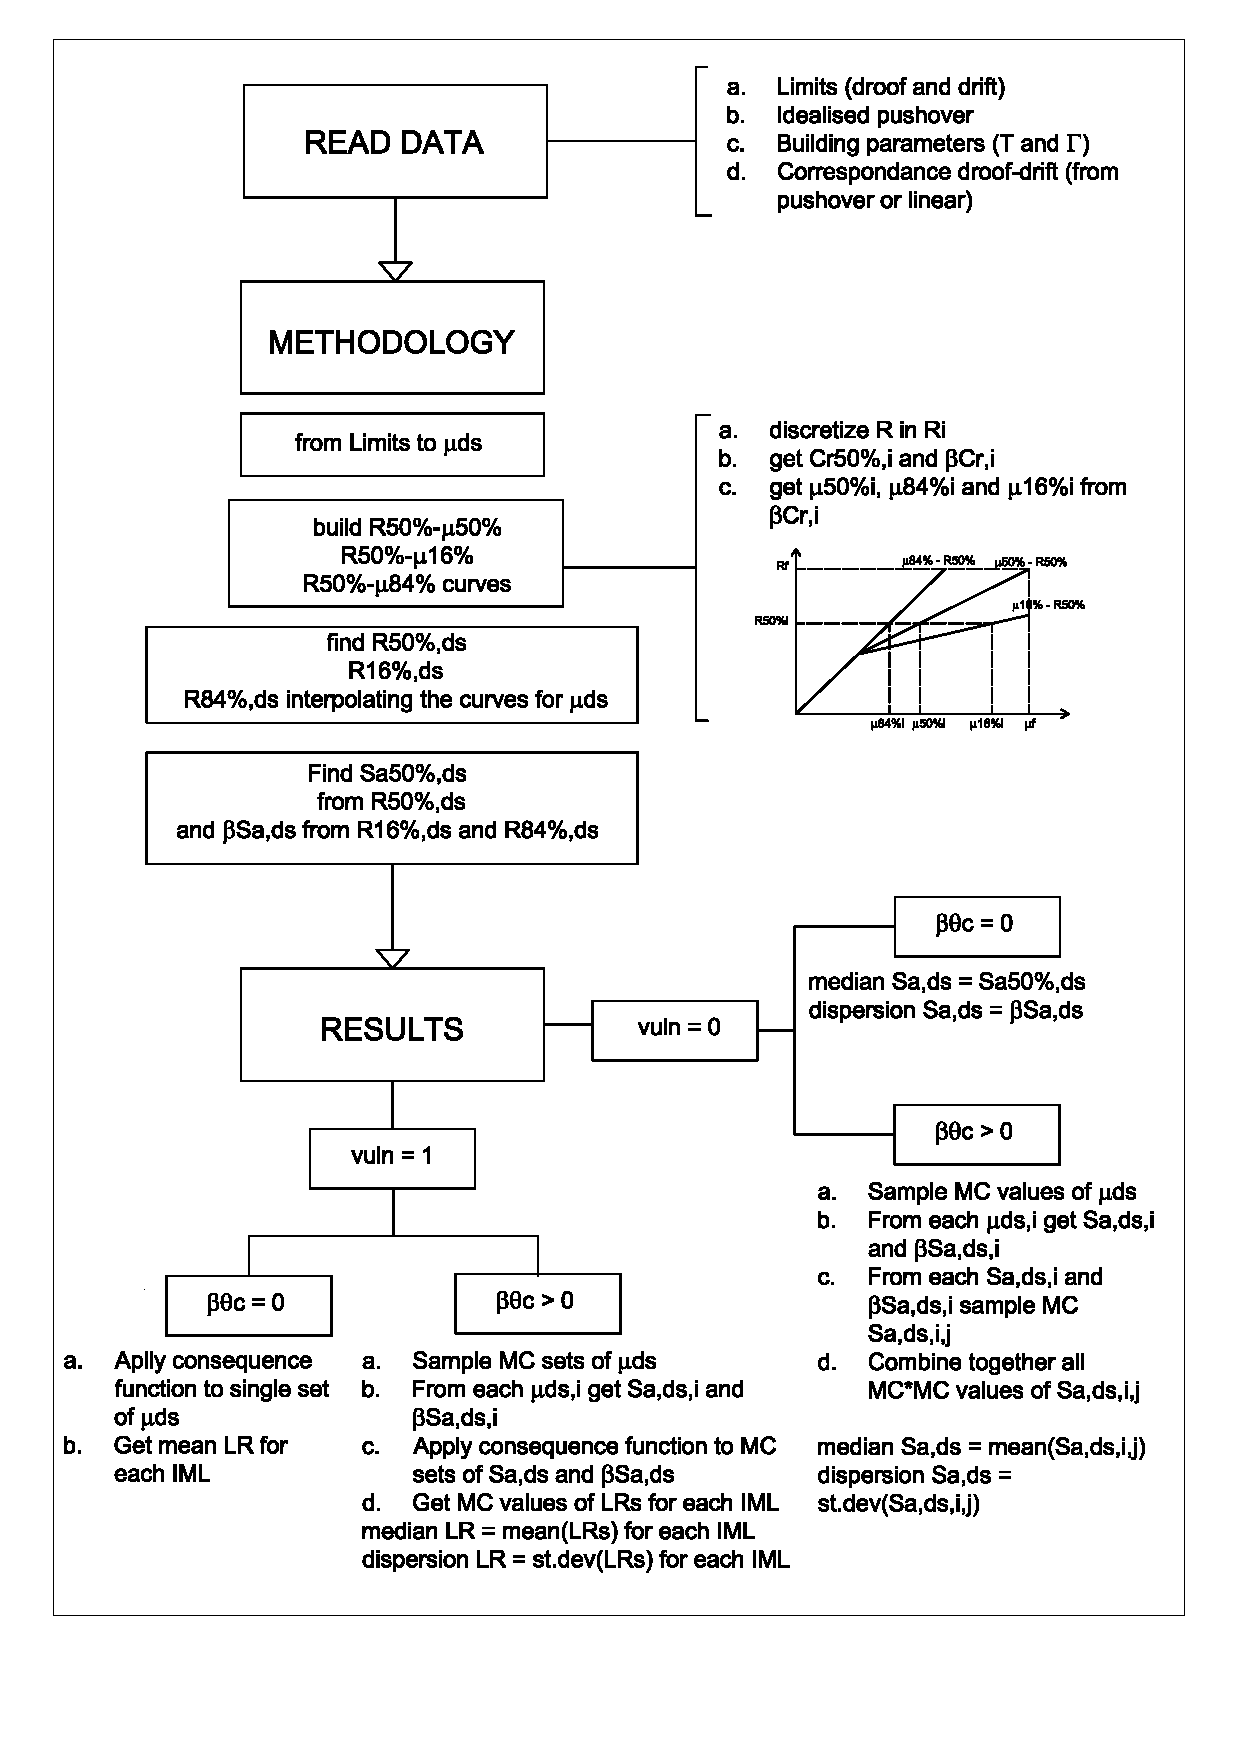
\includegraphics[width=15cm]{./figures/Cr-WorkFlow.jpg}
\caption{C$_R$-based procedure workflow.}
\label{fig:Cr_workflow}
\end{figure}

The option \textit{an\_type} must be set equal to 0 and the option \textit{in\_type} according to the input at disposal. The corresponding inputs should follow the requirements described in section \ref{subsubsec:InputCr}. Given this options the code proceeds with the following steps:\\

\begin{enumerate}
\item \textbf{Process Inputs within \textit{read\_data}  function}\\
\begin{enumerate}
\item If \textit{in\_type} = 0 roof displacement at limit states and idealised pushover are read from \textit{displacement\_profile.csv} and \textit{idealised\_curve.csv} respectively. A one-to-one relationship between roof displacement and drift is assumed.
\item If \textit{in\_type} = 1 results from pushover analysis are extracted from \textit{displacements\_pushover.csv} and \textit{reactions\_pushover.csv}, and drift limit states from \textit{limits.csv}. The relationship between drift and roof displacement is given by the pushover inputs.\\
The idealised 	pushover curve is then derived in the \textit{idealisation} function, where the idealisation process is conducted according to FEMA-440. The elastic stiffness is defined as the 	tangent stiffness passing through the point of the pushover curve where 60\% of the maximum base shear is reached, and the perfectly plastic branch is set at an height equal to 	the maximum base shear. The yielding point is found as the interception between the elastic and the plastic branch.\\
\end{enumerate}

Period, modal participation factor, number of buildings constituting the building class, importance factor (weight) of the each building within the class, average period of the class and $S_a(T_{av})/S_a(T_{blg})$ ratio are also returned by the function \textit{read\_data} .\\

\item \textbf{Fragility curve methodology}\\
The parameters extracted are used in the \textit{simplified\_bilinear} function, within the \textit{fragility\_process} function, to derive ductility levels $\mu_{ds}$, median spectral acceleration $\hat{S}_{a,ds}$ and the total dispersion $\beta_{S_a}$ at each limit state through the following steps:

\begin{enumerate}

\item The idealised MDoF system is transformed into an equivalent SDoF system, using $\Gamma_1$.

\item Ductility levels $\mu_{ds}$ corresponding to each damage threshold, are defined.

\item $\mu_{50\%}$ - $R_{50\%}$, $\mu_{16\%}$ - $R_{50\%}$ and $\mu_{84\%}$ - $R_{50\%}$ relationships are computed, as described in \ref{subsubsec:single-building}.

\item $R_{50\%}$ is computed for the ductility limit states $\mu_{ds}$, interpolating the aforementioned curves, and C$_{R_{50\%}}$ is calculated by mean of equation \ref{eq:Cr_RGM}.

\item $\hat{S}_{a,ds}$ and the corresponding dispersion $\beta_{S_{a d}}$ due to record-to-record variability are computed using eq. \ref{eq:SaR} and \ref{eq:betaR} for each limit state.

\item If dispersion due to uncertainty in the limit state $\beta_{\theta c}$ is different from zero, different ductility limit states are sampled for each median ductility level $\mu_{ds}$. For each sampled ductilities the corresponding $\hat{S}_{a,ds}$ and $\beta_{S_{a d}}$ are found as described in steps (d) and (e), and MC random S$_a$ for each of the MC sampled ductility limit states are computed using $\hat{S}_{a,ds}$ and $\beta_{S_{a d}}$.\\

\end{enumerate}

\item \textbf{Fragility curve results}\\
If number of buildings = 1\\
\begin{enumerate}
\item If \textit{vuln} = 0
the final values of median and dispersion of the fragility curves, $\hat{S}_{a,ds}$ and $\beta_{S_a}$, are computed as the mean and the standard deviation of the MC$^2$ samples of S$_a$, if many $\mu_{ds}$ were sampled at step 2.f, otherwise they correspond to the $\hat{S}_{a,ds}$ and $\beta_{S_{a d}}$, including only record-to-record variability, obtained at step 2.e.
All median values of S$_{a, ds}$ are converted to mean values $\mu_{ln(S_{a, ds})}$; mean $\mu_{ln(S_{a})}$ and total dispersion $\beta_{S_a}$ are then converted to logarithmic mean $\mu_{S_a}$ and logarithmic covariance $cov_{S_a}$, according to equations \ref{eq:median-to-mean} and \ref{eq:dispersion-to-standard} respectively.
Fragility curves for the building are displayed if the variable \textit{plotflag}[2] = 1, and logarithmic $\mu_{S_a}$ and $cov_{S_a}$ are exported in the \textit{outputs} folder.

\item 
If \textit{vuln} =1 if many values were sampled to account for uncertainty in the damage criteria at step 2.f, MC values of loss ratio LRs are defined for the MC sets of $\mu_{ds}$, using the \textit{damage\_to\_loss} function, for each intensity measure level defined in the variable \textit{iml} . Mean and standard deviation of LRs(iml), $\mu_{LR}$ and $\beta_{LR}$, are computed. If $\beta_{\theta c}$= 0 a single set of $\mu_{ds}$ is considered, resulting in no uncertainty in the LR for each iml.
Vulnerability curve for the building is displayed if the variable \textit{plotflag}[3] = 1, and $\mu_{LR}$ and $cov_{LR}$ at each iml are exported in the \textit{outputs} folder.\\

\end{enumerate}

If number of buildings > 1\\
\begin{enumerate}
\item If \textit{vuln} = 0
the final values of median and dispersion of the fragility curves, $\hat{S}_{a,ds}$ and $\beta_{S_a}$, are computed as the mean and the standard deviation of the MC$^2$ samples of S$_a$, if many $\mu_{ds}$ were sampled at step 2.f, otherwise they correspond to the $\hat{S}_{a,ds}$ and $\beta_{S_{a d}}$, including only record-to-record variability, obtained at step 2.e.

All $\hat{S}_{a, ds, blg}(T_1)$ are converted to mean values $\mu_{ln(S_{a, ds, blg})}(T_1)$ and then to the intensity measure in common with the rest of the buildings, $\mu_{ln(S_{a, ds, blg}(T_{av}))}$, according to eq. \ref{eq:Sa(Tav)}.\\
The $\mu_{ln(S_{a, ds, blg}(T_{av}))}$ are finally combined in a single lognormal curve for the building class, as described in section \ref{subsubsec:multiple-buildings}. 

Mean $\mu_{ln(S_{a})}$ and total dispersion $\beta_{S_a}$ are then converted to logarithmic mean $\mu_{S_a}$ and logarithmic covariance $cov_{S_a}$, according to equations \ref{eq:median-to-mean} and \ref{eq:dispersion-to-standard} respectively.

Fragility curves for the class of buildings are displayed if the variable \textit{plotflag}[2] = 1, and logarithmic $\mu_{S_a}$ and $cov_{S_a}$ are exported in the \textit{outputs} folder.

\item 
If \textit{vuln} =1
all $\hat{S}_{a, ds}(T_1)$ for each building are converted to mean $\mu_{ln(S_{a, ds})}(T_1)$ and then to the intensity measure in common with the rest of the buildings, $\mu_{ln(S_{a, ds, blg}(T_{av}))}$, according to eq. \ref{eq:Sa(Tav)}.

if many values were sampled to account for uncertainty in the damage criteria at step 2.f, MC values of loss ratio LRs are defined for the MC sets of $\mu_{ds}$, using the \textit{damage\_to\_loss} function, for each intensity measure level defined in the variable \textit{iml}. Mean and standard deviation of LRs(iml), $\mu_{LR}$ and $\beta_{LR}$, are computed. If $\beta_{\theta c}$= 0 a single set of $\mu_{ds}$ is considered, resulting in no uncertainty in the LR for each iml.
The $\mu_{LR, iml, blg}$ are finally combined in a single mean and standard deviations, as described in section \ref{subsubsec:multiple-buildings}. Vulnerability curve for the class of buildings is displayed if the variable \textit{plotflag}[3] = 1, and $\mu_{LR}$ and $cov_{LR}$ at each iml are exported in the \textit{outputs} folder.

\end{enumerate}

\end{enumerate}


		\subsection{spo2ida-based procedure (Vamvatsikos and Cornell, 2006)}
		\label{subsec:nls-spo2ida}
		The aim of this procedure is the estimation of the median spectral acceleration value $\hat{S}_{a,ds}$, that brings the structure to the attainment of a set of damage states ds, and the corresponding dispersion beta $\beta_{S_a}$, the parameters needed for the mathematical representation of fragility in equation \ref{eq:fragility-definition}. The aim is achieved making use of the tool spo2ida (Vamvatsikos and Cornell, 2006), where static pushover curves are converted into 16\%, 50\% and 84\% IDA curves, using empirical relationships from a large database of incremental dynamic analysis results, as shown in Figure~\ref{fig:spo2ida}.

\begin{figure}[H]
\centering
\includegraphics[width=12cm,height=8cm]{./figures/spo2ida.jpg}
\caption{spo2ida tool: IDA curves derived from Pushover curve.}
\label{fig:spo2ida}
\end{figure}

The spo2ida-based procedure presented herein is applicable to any kind of multi-linear capacity curve, and it is suitable for single building fragility curve estimation, as described in section \ref{subsubsec:single-building-spo2ida}. However the fragility curves derived for single buildings can be combined in a unique fragility curve, which considers the inter-building uncertainty, as described in section \ref{subsubsec:multiple-building-spo2ida}.

\subsubsection{Single-building Fragility and Vulnerability function}
\label{subsubsec:single-building-spo2ida}
Given the idealised capacity curve the spo2ida tool uses an implicit R-$\mu$-T relation to correlate nonlinear displacement, expressed in terms of ductility $\mu$ to the corresponding medians capacity in terms of the parameters R. R is the lateral strength ratio, defined as the ratio between the spectral spectral acceleration S$_a$ and the yielding capacity of the system S$_{ay}$. 

Each branch of the capacity curve, hardening, softening and residual plateau, is converted to a corresponding branch of the three ida curves, using the R-$\mu$-T relation, which is a function of the hardening stiffness, the softening stiffness and the residual force. These parameters are derived from the idealised pushover capacity expressed in $\mu$-R terms, as well as the ductility levels at the onset of each branch. If some of the branches of the pushover curve are missing because of the seismic behaviour of the system, spo2ida can equally work with bilinear, trilinear and quadrilinear idealisations.

The result of the spo2ida routine is thus a list of ductility levels and corresponding R values at 50\%, 16\% and 84\% percentiles. The distribution of R values at each ductility level, due to the record-to-record variability, is assumed to be lognormal and it can be easily converted to the dispersion of the lognormal distribution with the following equation:

\begin{equation}
\beta_{R(\mu)} = \frac{\ln R(\mu)_{84\%} - \ln R(\mu)_{16\%}}{2}
\label{eq:betaR}
\end{equation} 

$\beta_{R(\mu)}$ represents also the record-to-record variability of S$_a$ at different ductility levels $\beta_{S_a, d}$. Median R and its dispersion at ductility levels corresponding to the damage thresholds can thus be determined, and $\hat{S}_{a,ds}$ can be easily extracted simply multiplying $R_{50\%}(\mu_{ds})$ by the yielding capacity of the system $S_{ay}$, as shown in the following equation:

\begin{equation}
\hat{S}_{a,ds} = R_{50\%}(\mu_{ds}) S_{ay}
\label{eq:SaR}
\end{equation}
\begin{equation}
S_{ay} = \frac{4 \pi^2 \delta_{roof,y}}{g \Gamma_1 T_1^1}
\end{equation}

Since $\hat{R}$ and $\hat{S}_{a}$ are proportional they share the same dispersion.

If dispersion due to uncertainty in the limit state definition $\beta_{\theta c}$ is different from zero it can not be combined directly with the record-to-record dispersion, but a Monte Carlo sampling of the limit state needs to be performed instead. Different values of ductility limit state are sampled from the  lognormal distribution with median the median value of the ductility limit state, and dispersion the input $\beta_{\theta c}$. For each of these ductilities the corresponding R$_{16\%}$-R$_{50\%}$-R$_{84\%}$ are found and converted into $\hat{S}_{a,ds}$ and $\beta_{\theta d}$ according to equation \ref{eq:SaR} and \ref{eq:betaR}. N random S$_a$ corresponding to the N sampled ductility limit states are computed, and their median and the dispersion are estimated. These parameters constitute the median $\hat{S}_{a,ds}$ and the total dispersion $\beta_{S_a}$ for the considered damage state. The procedure is repeated for each damage state.

To derive a discrete vulnerability function at certain intensity measure levels, the input damage-to-loss factors are applied to the probability of occurance of each damage state, extracted from the probability of exceedance of each damage state described by the set of fragility curves. 

If dispersion due to uncertainty in the limit state is different from zero a vulnerability function is derived for the N sets of sampled ductility limit states. It results in N loss ratios for each defined intensity measure levels. Finally a lognormal distribution of the loss ratios is assumed at each iml and the vulnerability curve is defined at each iml by the mean and the standard deviation of all the computed loss ratios.

\subsubsection{Multiple-Building Fragility and Vulnerability function}
\label{subsubsec:multiple-building-spo2ida}
If multiple buildings have been input to derive a set of fragility curves for a class of buildings all $\hat{S}_{a,blg}$ and $\beta_{S_a,blg}$ are combined in a single lognormal curve for each damage state. A minimum of 5 buildings should be considered to obtain reliable results for the class. The procedure to get $\mu_{S_a,tot}$ and $cov_{S_a,tot}$ for the class of building is the same described in section \ref{subsubsec:multiple-buildings}, but the $\hat{S}_{a,blg}$ and $\beta_{S_a,blg}$ are those derived from each sampled set of ductility limit state.

A single vulnerability curve can also be obtained, from the single building vulnerability curves. If no dispersion in the limit state is defined, the method is the same described in section \ref{subsubsec:multiple-buildings}. Otherwise a vulnerability curve is derived for each building as explained in section \ref{subsub:single-building-spo2ida}, considering the sampled set of ductility limit states, that is to say that the mean loss ratio and its standard deviation at each iml, $\mu_{LR,iml,blg}$ and $\sigma_{LR,iml,blg}$ respectively, are found for each building.
Finally the mean loss ratio and its standard deviation, $\mu_{LR,iml}$ and $\sigma_{LR,iml}$, are found for the entire class of buildings as the weighted mean of the single $\mu_{LR,iml,blg}$ and the weighted SRSS of the inter-building and intra-building standard deviation, the standard deviation of the single means $\mu_{LR,iml,blg}$ and the single dispersions $\sigma_{LR,iml,blg}$ respectively, as described in eq \ref{eq:combination-lognormals-sigma}, substituting loss ratio to spectral acceleration.

\subsubsection{Inputs}
\label{subsubsec:InputSpo2ida}
The inputs must be formatted as comma-separated value files (.csv), and saved in the folder \textit{input}, contained in the NSP directory. If any other environment different from Windows is used make sure that the "comma separated values Windows" is selected as saving option when creating the input files. 

If multiple buildings want to be analysed to consider the inter-building uncertainty the parameters relative to each building should be added as additional lines in the tables, as shown in the examples below, otherwise a single line must be input.

If the user has already at disposal an idealised multilinear pushover curve for each building, that is to say that the variable \textit{in\_type} has been set to 0, the following data need to be provided in the corresponding csv files:

\begin{enumerate}
\item First period of vibration $T_1$, corresponding modal participation factor $\Gamma_1$, normalised with respect to the roof displacement, and weight for the combination of different buildings, input in \textit{building\_parameters.csv}, as in section \ref{subsubsec:InputCr}, input n. 1.
	
\item Top displacement at each damage state threshold and corresponding dispersion $\beta_{\theta c}$ input in \textit{displacement\_profile.csv}, as in section \ref{subsec:InputCr}, input n. 2. 
	
\item Idealised pushover curve, input in \textit{idealised\_curve.csv} as shown below. The parameters needed to describe the idealised pushover curve are: yielding displacement d$_y$, displacement at the onset of degradation d$_s$, displacement at the onset of residual force d$_{min}$, ultimate displacement d$_u$, maximum force F$_{max}$, residual force F$_{min}$. These parameters are represented in Figure~\ref{fig:quadrilinear}.

\begin{figure}[H]
\centering
\includegraphics[width=12cm,height=8cm]{./figures/quadrilinear.jpg}
\caption{Idealisation of capacity curve using multilinear elasto-plastic form.}
\label{fig:quadrilinear}
\end{figure}

\begin{table}[H]
\centering
\begin{tabular}{|c|c|c|c|c|c|c|} \hline
\textbf{n.building} & \textbf{d$_y$} & \textbf{d$_s$} & \textbf{d$_{min}$} & \textbf{d$_u$} & \textbf{F$_{max}$} & \textbf{F$_{min}$} \\ \hline
1 & 0.09	& 0.3	& a & b & 523 & 430\\ \hline
2 & 0.12	& 0.35	 & a & b & 400 & 305\\ \hline	
\end{tabular}
\end{table}

\item Consequence model (loss ratio per each damage state) consistent with the defined set of damage states, input in \textit{consequence.csv}, as in section \ref{subsubsec:InputCr}, input n. 5.
	
\end{enumerate}

If these data are not available, \textit{in\_type} = 0 can be selected and the "raw" results from a pushover analysis can be input instead. The same data as in section \ref{subsubsec:InputCr} for \textit{in\_type} = 0 can be input.

\subsubsection{Calculation Steps}
The overall workflow of spo2ida-based procedure is summarised in this section. The option \textit{an\_type} must be set equal to 1 and the option \textit{in\_type} according to the input at disposal. The corresponding inputs should follow the requirements described in section \ref{subsec:InputSpo2ida}. At this point the code proceeds with the following steps:

\begin{enumerate}
\item 
\begin{enumerate}
\item If \textit{in\_type} = 0, the roof displacement at each limit state and the idealised pushover curve parameters are extracted from \textit{displacement\_profile.csv} and \textit{idealised\_curve.csv} respectively.

\item If \textit{in\_type} = 1 the results from a pushover analysis are extracted from \textit{displacements\_pushover.csv} and \textit{reactions\_pushover.csv} and drift limit states from {limits.csv}. The idealised pushover curve is then derived in the \textit{idealisation} function, where the idealisation process is conducted according to the Gem Analytical Vulnerability Guidelines.	\end{enumerate}

\item The parameters extracted are used to derive ductility levels $\mu_{ds}$, median spectral acceleration $\hat{S}_{a,ds}$ and the total dispersion $\beta_{S_a}$ at each damage threshold through the following steps:
\begin{itemize}
\item The idealised MDoF system is transformed into an equivalent SDoF system, using $\Gamma_1$, and SDoF capacity curve is  expressed in terms of $\mu$-R.

\item The variables for spo2ida tool are extracted from the capacity curve and they are used as input to get the 16\%-50\%-84\% ida curves.

\item The ductility levels $\mu_{ds}$ corresponding to each damage threshold are defined, and the corresponding R$_{16\%}$-R$_{50\%}$-R$_{84\%}$ are found in ida outputs.

\item $\hat{S}_{a,ds}$ and the corresponding dispersion $\beta_{S_{a, d}}$ are computed using eq.~\ref{eq:SaR} and eq.~\ref{eq:betaR}, respectively.

\item If dispersion due to uncertainty in the limit state $\beta_{\theta c}$ is different from zero different ductility limit states are sampled for each median ductility level $\mu_{ds}$ and corresponding values of $\hat{S}_{a,ds}$ and $\beta_{S_{a, d}}$ are computed, as described in section \ref{subsubsec:single-building-spo2ida}, but not yet combined together.

\end{itemize}

\item All $\hat{S}_{a, ds}(T_1)$ are converted to mean $\mu_{ln(S_{a, ds})}(T_1)$ and then to the intensity measure in common with the rest of the buildings, $\mu_{ln(S_{a, ds}(T_{av}))}$, according to eq. \ref{eq:Sa(Tav)}.

\item Step 2. and 3. are repeated for the number of input buildings.

\item
\begin{enumerate}

\item If vulnerability = 0: All $\hat{S}_{a,ds}$ and $\beta_{S_{a, d}}$ from all the buildings and all the sampled ductility limit states are combined in a single lognormal curve, as described in section \ref{subsubsec:single-building-spo2ida}. 
Mean $\mu_{ln(S_{a})}$ and total dispersion $\beta_{S_a}$ are then converted to logarithmic mean $\mu_{S_a}$ and logarithmic covariance $cov_{S_a}$, according to equations \ref{eq:median-to-mean} and \ref{eq:dispersion-to-standard} respectively.
Fragility curves for the class of buildings are displayed if the variable \textit{plotflag}[2] = 1, and logarithmic $\mu_{S_a}$ and $cov_{S_a}$ are exported in the \textit{outputs} folder.
\item If vulnerability =1:  
For the intensity measure levels defined in the variable \textit{iml} a value of loss ratio $\mu_{LR, iml, blg}$ is defined for each building and a standard deviation $\sigma_{LR, iml, blg}$, if dispersion due to uncertainty in the limit state $\beta_{\theta c}$ is different from zero. They are finally combined in a single mean and standard deviationas described in section \ref{subsubsec:multiple-building-spo2ida}. Vulnerability curve for the class of buildings is displayed if the variable \textit{plotflag}[3] = 1, and $\mu_{LR}$ and $cov_{LR}$ at each iml are exported in the \textit{outputs} folder.
\end{enumerate}

\end{enumerate}

		\subsection{$R-mu-T$-based procedure (Dolsek and Fajfar, 2004)}
		\label{subsec:nls-dolsek-fajfar}
		The aim of this procedure is the estimation of the median spectral acceleration value $\hat{S}_a$, that brings the structure to the attainment of a set of damage states, and the corresponding dispersion beta $\beta_{S_a}$, the parameters needed for the mathematical representation of fragility in equation \ref{eq:fragility-definition}. The aim is achieved making use of a R-$\mu$-T relationship, between reduction factor R, ductility $\mu$ and period T, which is based on the work of Dolsek and Fajfar (2004). The R-$\mu$-T-based procedure presented herein is applicable to any kind of multi-linear capacity curve, and it is suitable for single building fragility curve estimation, as described in section \ref{subsubsec:single-building-DF}. However the fragility curves derived for single buildings can be combined in a unique fragility curve, which considers also the inter-building uncertainty, as described in section \ref{subsubsec:multiple-building-DF}.

\subsubsection{Single Building Fragility and Vulnerability function}
\label{subsubsec:single-building-DF}
This procedure provides a simple relationship between median damage state threshold, expressed in terms of top displacement $\hat{d}_{roof, ds}$, at each damage state threshold \textit{ds}, and the corresponding median elastic Spectral acceleration value $\hat{S}_{a, ds}$, as explained in C$_{R}$-based procedure and reported in the following equation:

\begin{equation}
\hat{S}_{a,ds}(T_1) = \frac{4 \pi^2}{\hat{C}_R T^2 \Gamma_1 \Phi_1} \hat{d}_{roof, ds}
\label{eq:basic_DF}
\end{equation}

The value of C$_R$, the ratio between the inelastic and the elastic spectral displacement, is found from the following equation:

\begin{equation}
\hat{C}_{R} = \frac{\mu_{ds}}{R_{ds}}
\label{eq:Cr_DF}
\end{equation}

where $\mu_{ds}$ and $R_{ds}$ are the median values of ductility level and the reduction factor at the attainment of \textit{ds}. According to the results of an extensive parametric study using three different sets of recorded and semi-artificial ground motions, Dolsek and Fajfar (2004) related the ductility demand $\mu$ and reduction factor R through the following formula:

\begin{equation}
\label{eq:mu_DF}
\mu = \frac{1}{c} (R-R_{0})+\mu_{0}
\end{equation}

In the proposed model $\mu$ is linearly dependent on R within two reduction factor intervals. The parameter c defines the slope of the R–$\mu$ relation, and it depends on the initial period of the system T, the ratio r$_{u}$, the reduction factor R and the corner periods T$_{c}$ and T$_{d}$. T$_{c}$ and T$_{d}$ are the corner periods between the constant acceleration and constant velocity part of the idealised elastic spectrum, and between the constant velocity and constant displacement part of the idealised elastic spectrum respectively. $R_{0}$ and $\mu_{0}$ are the values of R and $\mu$ on the capacity curve corresponding to the hardening behaviour and the softening respectively.

Given the parameters of the multilinear pushover curves (R$_{\mu_{0}}$, $\mu_{0}$, r$_{u}$) and T, the median R - $\mu$ curve can be constructed using the aforementioned relationship. 
The relationship between the 16$^{th}$ and 84$^{th}$ fractiles of $\mu$ and R$_{50}$ needs to be derived using the equations from Ruiz-Garcia and Miranda instead, given that Dolsek and Fajfar do not provide estimates of the dispersion of R. This is done as in the C$_R$-based procedure by computing $\beta_{\theta d}$ for a number of R with eq. \ref{eq:beta_eq_RGM}, and obtaining from this value the 16$^{th}$ and 84$^{th}$ fractiles of $\mu$ ($\mu_{16\%}$ and $\mu_{84\%}$), according to the Equations \ref{eq:mu16-beta} and \ref{eq:mu84-beta}. The $\mu_{50\%}-R_{50\%}$, $\mu_{16\%}-R_50\%$ and $\mu_{84\%}-R_50\%$ curves can thus be drawn.\\

For each $\mu_{ds}$ the corresponding $R_{50\%}$, $R_{16\%}$, and $R_{84\%}$ values are found interpolating the aforementioned curves, and converted into $\hat{S}_{a,ds}$ and $\beta_{S_{a d}}$ according to equations \ref{eq:SaR} and \ref{eq:betaR}.

If dispersion due to uncertainty in the limit state definition $\beta_{\theta c}$ is different from zero it can be combined with the record-to-record dispersion either in a simplified way or with a Monte Carlo sampling procedure.\\

In the simplified method the dispersion of $S_a$ due to uncertainty in the damage state threshold $\beta_{S_{a c}}$ can be found converting the dispersion in the damage threshold $\beta_{\theta c}$, as explaind in section \ref{subsubsec:single-building} and reported in the following equation:

\begin{equation}
\beta_{S_{a c}} = \frac{1}{b} \beta_{\theta c}
\label{eq:betasc_DF}
\end{equation}

In order to derive the b values, which represent the slope of the R-$\mu$ relation in the log-space, a further step needs to be made, because the R-$\mu$-T is suggested by the authors as conservative, since it is not based on the median but on the mean $\mu$ given R. An attempt was made to correct it reducing the median R curve by 15\%, $R_{50\% corrected}$, as shown in equation \ref{eq:Rcorrected}, and extrapolating the corresponding $\mu_{50\% corrected}$.

\begin{equation}
R_{50\% corrected}=0.85 R_{50\%}
\label{eq:Rcorrected}
\end{equation}
\begin{equation}
b = \frac{ln(\mu_{50\% corrected})}{ln(R_{50\% corrected})}
\label{eq:bcorrected_DF}
\end{equation}

Finally the dispersion of $S_a$ due to record-to-record variability, can be combined with the dispersion of $S_a$ due to uncertainty in the damage state threshold, as in the following equation:

\begin{equation}
\beta_{S_a} = \sqrt{\beta_{S_{a c}}^2+\beta_{S_{a d}}^2}
\label{eq:betatot_DF}
\end{equation}

In the Monte Carlo approach different values of ductility limit state are sampled from the lognormal distribution with median the median value of the ductility limit state, and dispersion the input $\beta_{\theta c}$.
For each of these ductilities the corresponding $R_{50\%}$, $R_{16\%}$, and $R_{84\%}$ values are found interpolating the $\mu_{50\%}-R_{50\%}$, $\mu_{16\%}-R_50\%$ and $\mu_{84\%}-R_50\%$ curves, and converted into $\hat{S}_{a,ds}$ and $\beta_{S_{a d}}$ according to Equations \ref{eq:SaR} and \ref{eq:betaR}.

MC random S$_a$ for each of the MC sampled ductility limit states are computed using $\hat{S}_{a,ds}$ and $\beta_{S_{a d}}$, and their median and dispersion are estimated. These parameters constitute the median $\hat{S}_{a,ds}$ and the total dispersion $\beta_{S_a}$ for the considered damage state. The procedure is repeated for each damage state.

To derive a discrete vulnerability function at certain intensity measure levels, the input damage-to-loss factors are applied to the probability of occurance of each damage state, extracted from the probability of exceedance of each damage state described by the fragility function.
If dispersion due to uncertainty in the limit state is different from zero a vulnerability function is derived for the MC sets of sampled ductility limit states. It results in MC loss ratios for each defined intensity measure levels. Finally a lognormal distribution of the loss ratios is assumed at each iml with mean and standard deviation the mean and standard deviation of the all the computed LRs.

\subsubsection{Multiple Building Fragility and Vulnerability function}
\label{subsubsec:multiple-building-DF}
 If multiple buildings have been input to derive fragility function for a class of buildings all $\hat{S}_{a, blg}$ and $\beta_{S_a, blg}$ are combined in a single lognormal curve as described in section \ref{subsubsec:multiple-buildings}. The same holds for vulnerability function, as described in the same section.

\subsubsection{Inputs}
The data the user needs provided and the their format is described in section \ref{subsubsec:InputSpo2ida}

\subsubsection{Calculation Steps} 
The overall workflow of R-$\mu$-T-based procedure is summarised in this section and represented in Figure \ref{fig:Cr_workflow} for the case of a single building fragility/vulnerability function. 

\begin{figure}[!htbp]
\centering
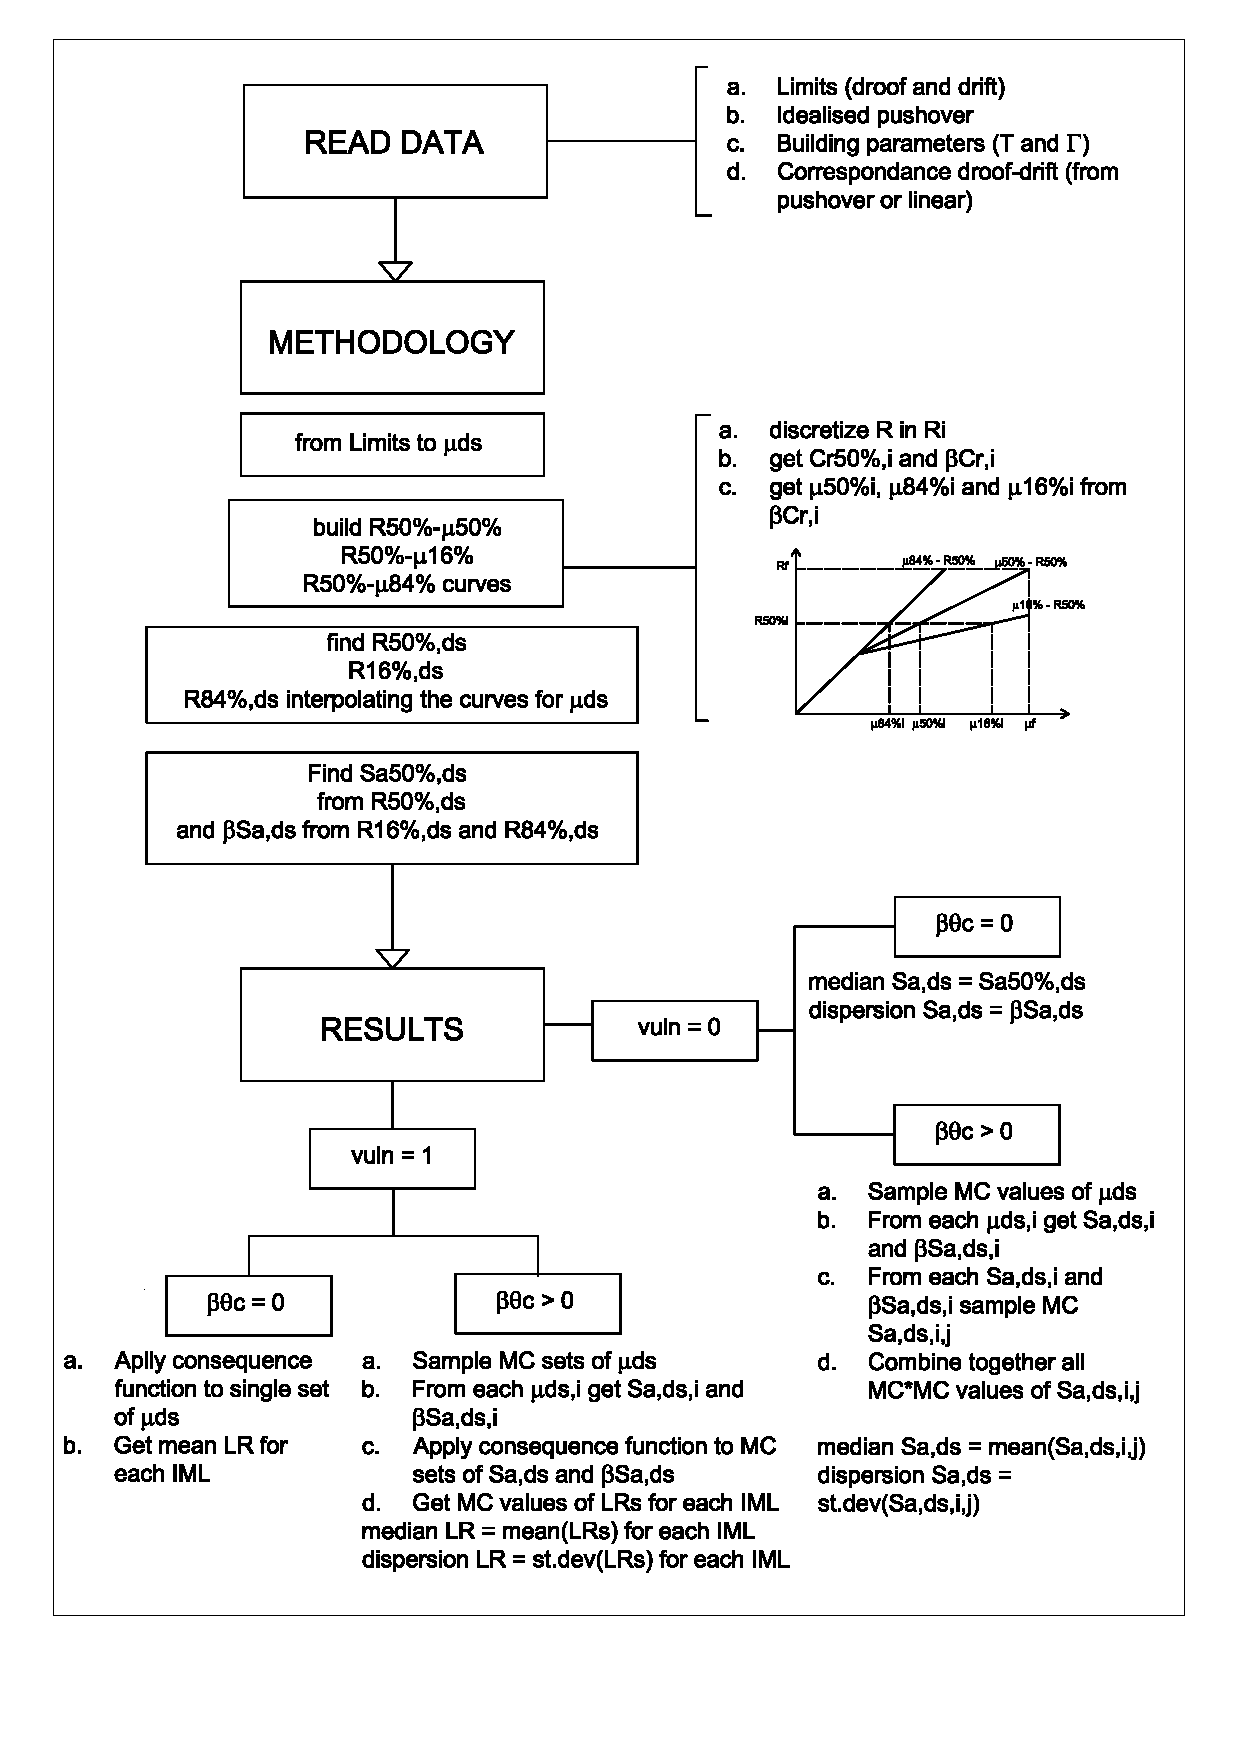
\includegraphics[width=15cm]{./figures/Cr-WorkFlow.jpg}
\caption{C$_R$-based procedure workflow.}
\label{fig:Cr_workflow}
\end{figure}

The option \textit{an\_type} must be set equal to 2 and the option \textit{in\_type} according to the input at disposal. The corresponding inputs should follow the requirements described in section \ref{subsubsec:InputSpo2ida}.Given these options the code proceeds with the following steps:\\

\begin{enumerate}
\item \textbf{Process Inputs within \textit{read\_data}  function}\\

\begin{enumerate}
\item If \textit{in\_type} = 0, the roof displacement at each limit state and the idealised pushover curve parameters are extracted from \textit{displacement\_profile.csv} and \textit{idealised\_curve.csv} respectively. A one-to-one relationship between roof displacement and drift is assumed
\item If \textit{in\_type} = 1 the results from a pushover analysis are extracted from \textit{displacements\_pushover.csv} and \textit{reactions\_pushover.csv} and drift limit states from {limits.csv}. The relationship between roof displacement and drift is given by the pushover inputs. The idealised pushover curve is then derived in the \textit{idealisation} function, where the idealisation process is conducted according to the Gem Analytical Vulnerability Guidelines.\\
\end{enumerate}

Period, modal participation factor, number of buildings constituting the building class, importance factor (weight) of the each building within the class, average period of the class and $S_a(T_{av})/S_a(T_{blg})$ ratio are also returned by the function \textit{read\_data} .\\

\item \textbf{Fragility curve methodology}\\
The parameters extracted are used in the \textit{DF\-fragility} function, within the \textit{fragility\_process} function, to derive ductility levels $\mu_{ds}$, median spectral acceleration $\hat{S}_{a,ds}$ and the total dispersion $\beta_{S_a}$ at each limit state through the following steps:

\begin{enumerate}

\item The idealised MDoF system is transformed into an equivalent SDoF system, using $\Gamma_1$, and the SDoF capacity curve is expressed in terms of $\mu$ and R.

\item Ductility levels $\mu_{ds}$ corresponding to each damage threshold, are defined.

\item The input variables R$_{\mu_{0}}$, $\mu_{0}$, r$_{u}$ for Equation \ref{eq:mu_DF} are inferred from the capacity curve and median $\mu$ - R relationship is computed using Equation \ref{eq:mu_DF}.

\item $\mu_{16\%}$ - $R_{50\%}$ and $\mu_{84\%}$ - $R_{50\%}$ relationships are computed as in C$_R$-based procedure.

\item $R_{50\%}$, $R_{16\%}$ and $R_{84\%}$ is computed for the ductility limit states $\mu_{ds}$, interpolating the aforementioned R - $\mu$ curves.

\item $\hat{S}_{a,ds}$ and the corresponding dispersion $\beta_{S_{a d}}$ due to record-to-record variability are computed using eq. \ref{eq:SaR} and \ref{eq:betaR} for each limit state.

\item If dispersion due to uncertainty in the limit state $\beta_{\theta c}$ is different from zero, different ductility limit states are sampled for each median ductility level $\mu_{ds}$. For each sampled ductilities the corresponding $\hat{S}_{a,ds}$ and $\beta_{S_{a ds}}$ are found as described in steps from (d) to (f), and MC random S$_a$ for each of the MC sampled ductility limit states are computed using $\hat{S}_{a,ds}$ and $\beta_{S_{a d}}$.\\

\end{enumerate}

\item \textbf{Fragility curve results}\\
If number of buildings = 1\\
\begin{enumerate}
\item If \textit{vuln} = 0
the final values of median and dispersion of the fragility curves, $\hat{S}_{a,ds}$ and $\beta_{S_a}$, are computed as the mean and the standard deviation of the MC$^2$ samples of S$_a$, if many $\mu_{ds}$ were sampled at step 2.g, otherwise they correspond to the $\hat{S}_{a,ds}$ and $\beta_{S_{a d}}$, including only record-to-record variability, obtained at step 2.f.

All median values of $S_{a, ds}$ are converted to mean values $\mu_{ln(S_{a, ds})}$; mean $\mu_{ln(S_{a})}$ and total dispersion $\beta_{S_a}$ are then converted to logarithmic mean $\mu_{S_a}$ and logarithmic covariance $cov_{S_a}$, according to equations \ref{eq:median-to-mean} and \ref{eq:dispersion-to-standard} respectively.

Fragility curves for the building are displayed if the variable \textit{plotflag}[2] = 1, and logarithmic $\mu_{S_a}$ and $cov_{S_a}$ are exported in the \textit{outputs} folder.

\item 
If \textit{vuln} =1
if many values were sampled to account for uncertainty in the damage criteria at step 2.f, MC values of loss ratio LRs are defined for the MC sets of $\mu_{ds}$, using the \textit{damage\_to\_loss} function, for each intensity measure level defined in the variable \textit{iml}. Mean and standard deviation of LRs(iml), $\mu_{LR}$ and $\beta_{LR}$, are computed. If $\beta_{\theta c}$= 0 a single set of $\mu_{ds}$ is considered, resulting in no uncertainty in the LR for each iml.
Vulnerability curve for the building is displayed if the variable \textit{plotflag}[3] = 1, and $\mu_{LR}$ and $cov_{LR}$ at each iml are exported in the \textit{outputs} folder.\\

\end{enumerate}

If number of buildings > 1\\
\begin{enumerate}
\item If \textit{vuln} = 0
the final values of median and dispersion of the fragility curves, $\hat{S}_{a,ds}$ and $\beta_{S_a}$, are computed as the mean and the standard deviation of the MC$^2$ samples of S$_a$, if many $\mu_{ds}$ were sampled at step 2.g, otherwise they correspond to the $\hat{S}_{a,ds}$ and $\beta_{S_{a d}}$, including only record-to-record variability, obtained at step 2.f.

All $\hat{S}_{a, ds, blg}(T_1)$ are converted to mean $\mu_{ln(S_{a, ds, blg})}(T_1)$ and then to the intensity measure in common with the rest of the buildings, $\mu_{ln(S_{a, ds, blg}(T_{av}))}$, according to eq. \ref{eq:Sa(Tav)}.\\
The $\mu_{ln(S_{a, ds, blg}(T_{av}))}$ are finally combined in a single lognormal curve for the building class, as described in section \ref{subsubsec:multiple-buildings}. 

Mean $\mu_{ln(S_{a})}$ and total dispersion $\beta_{S_a}$ are then converted to logarithmic mean $\mu_{S_a}$ and logarithmic covariance $cov_{S_a}$, according to equations \ref{eq:median-to-mean} and \ref{eq:dispersion-to-standard} respectively.

Fragility curves for the class of buildings are displayed if the variable \textit{plotflag}[2] = 1, and logarithmic $\mu_{S_a}$ and $cov_{S_a}$ are exported in the \textit{outputs} folder.

\item 
If \textit{vuln} =1
all $\hat{S}_{a, ds}(T_1)$ for each building are converted to mean $\mu_{ln(S_{a, ds})}(T_1)$ and then to the intensity measure in common with the rest of the buildings, $\mu_{ln(S_{a, ds, blg}(T_{av}))}$, according to eq. \ref{eq:Sa(Tav)}.

For each intensity measure level defined in the variable \textit{iml} MC values of loss ratio LRs are defined for the MC sets of $\mu_{ds}$, if many values were sampled to account for uncertainty in the damage criteria at step 2.f, using the \textit{damage\_to\_loss} function. Mean and standard deviation of LRs(iml), $\mu_{LR}$ and $\beta_{LR}$, are computed. If $\beta_{\theta c}$= 0 a single set of $\mu_{ds}$ is considered, resulting in no uncertainty in the LR for each iml.\\

The $\mu_{LR, iml, blg}$ are finally combined in a single mean and standard deviations, as described in section \ref{subsubsec:multiple-buildings}. Vulnerability curve for the class of buildings is displayed if the variable \textit{plotflag}[3] = 1, and $\mu_{LR}$ and $cov_{LR}$ at each iml are exported in the \textit{outputs} folder.

\end{enumerate}

\end{enumerate}



		\subsection{NLS methods without record-to-record dispersion}
		\label{subsec:nls-no-dispersion}
		\input{./tex/nls-no-dispersion}

	\section{Non-linear Dynamic (NLD) Methods}
	\label{sec:nld-intro}
	Nonlinear Dynamic Methods are based on the results of many dynamic analyses, which relate the seismic response of a structure, represented by an Engineering Demand Parameter (EDP), like maximum top displacement, maximum inter-storey drift ratio, maximum top drift etc., to the Intensity Measure Level (IML) of the input accelerograms. 
Many methods exists in literature to perform a series of dynamic analysis and to post-process the results in order to derive fragility curves. Some of them treat a single building to estimate directly the median seismic intensity value corresponding to the attainment of different damage state threshold (limit state), and the corresponding dispersion (Vamvatsikos and Cornell, 2002, Ellingwood and Kinali, 2009). Others treat a class of buildings, and lead to the evaluation of the probabilities of different damage states for a series of IMLs and thus to the set up of a damage probability matrix (Singhal and Kiremidjian, 1996, Silva et al., 2013).

The last approach have been implemented in the DPM-based procedure, explained in section \ref{sec:DPM}, from the point of view of the necessary scientific background behind and their step-by-step implementation in the python script.

		\subsection{Using the NLD module}
		\label{subsec:nld-how-to-use}
		To start using the nonlinear dynamic method a command line text editor should be used to enter manually the folder location where the \textit{rmtk} has been saved, as shown in the example below:

\begin{Verbatim}[frame=single, commandchars=\\\{\}, samepage=true]
cd path/to/rmtk/folder/rmtk/vulnerability
\end{Verbatim}

Where /path/to/rmtk/folder/ is the system path to the location of the \textit{rmtk} folder. From the text editor iPython browser page can be opened with the following command line:

\begin{Verbatim}[frame=single, commandchars=\\\{\}, samepage=true]
ipython-2.7 notebook --pylab=inline
\end{Verbatim}

Once the iPython page is opened on the browser, the python scripts contained in the \textit{rmtk} directory will be visible. The file \textit{NDM.ipynb} should be selected to start the calculations.

In the initial section of the script "Define Options" the user needs to set the options and to enter the input corresponding to the defined options in the folder \textit{NDP/input}. In section~\ref{subsubsec:NDMoptions} the alternatives values that the initial variables can assume and their meaning are described in detail, while the parameters to be inserted in the input files are fully described in section~\ref{subsubsec:NDMinputs}.

		\subsection{Damage probability matrix DPM-based procedure}
		\label{subsec:nld-dpm}
		\input{./tex/nld-dpm}

		\subsection{Post-processing IDA}
		\label{subsec:nld-ida}
		\input{./tex/nld-ida}

		% \subsection{Multiple stripe analysis (Jalayer, 2003)}
		% \label{subsec:nld-msa}
		% \input{./tex/nld-msa}

%----------------------------------------------------------------------------------------
%	CHAPTER 3
%----------------------------------------------------------------------------------------
\chapterimage{./figures/chapter_head_2.pdf} % Chapter heading image
\chapter{Plotting}
\label{chap:plotting}


%----------------------------------------------------------------------------------------
%	BIBLIOGRAPHY
%----------------------------------------------------------------------------------------
% \include{./book/bibliography}


%----------------------------------------------------------------------------------------
%	INDEX
%----------------------------------------------------------------------------------------

\cleardoublepage
\phantomsection
\setlength{\columnsep}{0.75cm}
\addcontentsline{toc}{chapter}{\textcolor{ocre}{Index}}
\printindex
\printglossary


%----------------------------------------------------------------------------------------
%	APPENDICES
%----------------------------------------------------------------------------------------
%\part{Appendices}
\appendix
\chapterimage{./figures/chapter_head_2.pdf} % Chapter heading image
\chapter{The 10 Minute Guide to Python!}
\label{sec:python_guide}
% \begin{myfancybox}
% The objectives of this chapter are:
% \begin{itemize}
%     \item To introduce Python data types to facilitate use of the RMTK for Python beginners
% \end{itemize}
% \end{myfancybox}
\input{./tex/python-guide.tex}


\end{document}